%  LaTeX support: latex@mdpi.com 
%  For support, please attach all files needed for compiling as well as the log file, and specify your operating system, LaTeX version, and LaTeX editor.

%=================================================================
\documentclass[futureinternet,article,submit,pdftex,moreauthors]{Definitions/mdpi} 

%--------------------
% Class Options:
%--------------------
%----------
% journal
%----------
% Choose between the following MDPI journals:
% For posting an early version of this manuscript as a preprint, you may use "preprints" as the journal. Changing "submit" to "accept" before posting will remove line numbers.

%---------
% article
%---------

%----------
% submit
%----------
% The class option "submit" will be changed to "accept" by the Editorial Office when the paper is accepted. This will only make changes to the frontpage (e.g., the logo of the journal will get visible), the headings, and the copyright information. Also, line numbering will be removed. Journal info and pagination for accepted papers will also be assigned by the Editorial Office.

%------------------
% moreauthors
%------------------
% If there is only one author the class option oneauthor should be used. Otherwise use the class option moreauthors.

%---------
% pdftex
%---------
% The option pdftex is for use with pdfLaTeX. Remove "pdftex" for (1) compiling with LaTeX & dvi2pdf (if eps figures are used) or for (2) compiling with XeLaTeX.

%=================================================================
% MDPI internal commands - do not modify
\firstpage{1} 
\makeatletter 
\setcounter{page}{\@firstpage} 
\makeatother
\pubvolume{1}
\issuenum{1}
\articlenumber{0}
\pubyear{2024}
\copyrightyear{2024}
%\externaleditor{Academic Editor: Firstname Lastname}
\datereceived{ } 
\daterevised{ } % Comment out if no revised date
\dateaccepted{ } 
\datepublished{ } 
%\datecorrected{} % For corrected papers: "Corrected: XXX" date in the original paper.
%\dateretracted{} % For corrected papers: "Retracted: XXX" date in the original paper.
\hreflink{https://doi.org/} % If needed use \linebreak
%\doinum{}
%\pdfoutput=1 % Uncommented for upload to arXiv.org
%\CorrStatement{yes}  % For updates


%=================================================================
% Add packages and commands here. The following packages are loaded in our class file: fontenc, inputenc, calc, indentfirst, fancyhdr, graphicx, epstopdf, lastpage, ifthen, float, amsmath, amssymb, lineno, setspace, enumitem, mathpazo, booktabs, titlesec, etoolbox, tabto, xcolor, colortbl, soul, multirow, microtype, tikz, totcount, changepage, attrib, upgreek, array, tabularx, pbox, ragged2e, tocloft, marginnote, marginfix, enotez, amsthm, natbib, hyperref, cleveref, scrextend, url, geometry, newfloat, caption, draftwatermark, seqsplit
% cleveref: load \crefname definitions after \begin{document}

%PLACE TO ADD COMMANDS
\usepackage{lipsum}
\usepackage{algorithm}
\usepackage{algpseudocode}
\usepackage{subcaption}

%=================================================================
% Please use the following mathematics environments: Theorem, Lemma, Corollary, Proposition, Characterization, Property, Problem, Example, ExamplesandDefinitions, Hypothesis, Remark, Definition, Notation, Assumption
%% For proofs, please use the proof environment (the amsthm package is loaded by the MDPI class).

%=================================================================
% Full title of the paper (Capitalized)
\Title{A Lightweight AI-based  Approach For Drone Jamming Detection}

% MDPI internal command: Title for citation in the left column
\TitleCitation{A Lightweight AI-based  Approach For Drone Jamming Detection}

% Author Orchid ID: enter ID or remove command
\newcommand{\orcidauthorA}{0009-0001-6239-0572} % Add \orcidA{} behind the author's name
\newcommand{\orcidauthorB}{0000-0002-0267-4733} % Add \orcidB{} behind the author's name
\newcommand{\orcidauthorC}{0000-0001-6271-7988}

% Authors, for the paper (add full first names)
\Author{Sergio Cibecchini*\orcidA{}, Francesco Chiti $^{1}$\orcidB{} and Laura Pierucci$^{2}$\orcidC{}}

%\longauthorlist{yes}

% MDPI internal command: Authors, for metadata in PDF
\AuthorNames{Sergio Cibecchini, Francesco Chiti and Laura Pierucci}

% MDPI internal command: Authors, for citation in the left column
\AuthorCitation{Cibecchini, S.; Chiti, F.; Pierucci, L.}
% If this is a Chicago style journal: Lastname, Firstname, Firstname Lastname, and Firstname Lastname.

% Affiliations / Addresses (Add [1] after \address if there is only one affiliation.)
\address {
$^{1}$ \quad Dipartimento di Ingegneria dell'Informazione, Università degli Studi di Firenze, Florence, Italy; francesco.chiti@unifi.it\\
$^{2}$ \quad Dipartimento di Ingegneria dell'Informazione, Università degli Studi di Firenze, Florence, Italy; laura.pierucci@unifi.it\\
}


% Contact information of the corresponding author
\corres{Correspondence: sergio.cibecchini@edu.unifi.it}

% Current address and/or shared authorship
%\firstnote{Current address: Affiliation.}  % Current address should not be the same as any items in the Affiliation section.
%\secondnote{These authors contributed equally to this work.}
% The commands \thirdnote{} till \eighthnote{} are available for further notes

%\simplesumm{} % Simple summary

%\conference{} % An extended version of a conference paper

% Abstract (Do not insert blank lines, i.e. \\) 
\abstract{The future integration of drones in 6G networks will significantly enhance their capabilities, enabling a wide range of new applications based on autonomous operation. However, drone networks are particularly vulnerable to Jamming attacks, a type of Availability attack that can disrupt network operation and hinder drone functionality. In this paper, we propose a low complexity unsupervised machine learning approach for the detection of constant and periodic jamming attacks, using the Isolation Forest algorithm. We detail the tuning of the base model as well as the integration with a Majority Rule module which significantly reduced the number of false positives caused by environmental noise, achieving high accuracy and precision. Our approach outperforms the standard Isolation Forest model in the detection of both constant and periodic jamming attacks, while still correctly identifying nominal traffic. Finally, we discuss the potential integration of the proposed solution in 6G-enabled drone networks, as a lightweight edge-based solution for enhancing security against jamming attacks. }

% Keywords
\keyword{Jamming attacks, 6G Drone Networks, Isolation Forest, Edge AI, IoT Security} 

% The fields PACS, MSC, and JEL may be left empty or commented out if not applicable
%\PACS{J0101}
%\MSC{}
%\JEL{}


%%%%%%%%%%%%%%%%%%%%%%%%%%%%%%%%%%%%%%%%%%
\begin{document}

%%%%%%%%%%%%%%%%%%%%%%%%%%%%%%%%%%%%%%%%%%
%\setcounter{section}{-1} %% Remove this when starting to work on the template.
\section{Introduction}

The shift from 4G to 5G has been a generational leap and has revolutionized connectivity. 
Despite 5G still being in its early stages of adoption at the time of writing \cite{5GStatisticsTaylor}, the research community is already working on the next generation of wireless communication technologies, 6G. 
6G technology is expected to enable a wide variety of new use cases, thanks to massive coverage as well as improvements in both data rates and latency, especially for IoT domains~\cite{ChFaPi21}. All of these advancements will in turn bring forth new security challenges specific to those applications. 

One of the main differences between 5G and 6G technology will be a much deeper integration with Artificial Intelligence (AI). While Software Defined Networks (SDN) have played a key role in improving the efficiency and security 
of 5G networks, 6G is expected to take this a step further, with the networks being designed to be AI native from the ground up. This is what the authors of \cite{6GRoadmapLetaief} define as 
the shift from \textit{Softwarization} to \textit{Intelligentization}. 

AI integration in 6G networks will greatly strengthen the security of the network against potential threats. 
By leveraging Diagnostic Analytics, a collection of insights into the status of the network, security teams 
will be able to train specific AI models to detect and respond to security threats in real-time.

In this paper we focus on a specific aspect of the security of 6G networks, namely we provide a lightweight edge-based Machine Learning approach 
for the detection of jamming attacks in networks of drones. We conceptualize a scenario where a drone is subject to constant and periodic jamming and has to rely on an internal AI model to detect the attack and apply the appropriate countermeasures. 

In the future, IoT devices are expected to come equipped with AI-specific chips that will allow them to run AI models directly on the edge, without the need to offload computation to a central server. This approach, aligning with the context-aware autonomic computing and communications paradigm~\cite{ChFaLoPu16}, is especially useful in the case of jamming attacks, where the communication between the device and the server is disrupted.
Our solution is designed to run on a resource-constrained IoT device like a drone and to be lightweight, both in terms of memory usage and computational power.
Despite the low resource requirements, the proposed approach is able to detect both constant and periodic jamming attacks with a high degree of accuracy, as well as correctly classify normal traffic. 

The paper is organized in five Sections: 
\begin{enumerate}
	\item \textbf{Topic overview:} General overview of the benefits of drone integration in 6G networks, analysis of jamming attacks: types, mitigation and detection. Discussion of the advantages provided by an edge AI approach for jamming detection. 
	\item \textbf{System Model:} Description of the analyzed scenario, along with the dataset, algorithms, and evaluation metrics chosen for the tests.
	\item \textbf{Model Performance:} Explanation of the testing methodology, including model tuning, testing phases, and detailed description of the performance of the model.
	\item \textbf{Discussion:} Analysis of the results from the previous section and the advantages of the proposed approach.
	\item \textbf{Conclusions:} Overview of how the proposed solution applies to real-world scenarios, with a discussion on potential future research directions.
\end{enumerate}

\section{Related Works}

Detection of jamming attacks in wireless networks has been a topic of interest for the research community for many years. A wide variety of approaches have been proposed for different types of networks, with most of the work focusing on the detection of jamming attacks in Vehicular Ad-Hoc Networks (VANETs)\cite{VANETsAI-Lyamin}.

The authors of \cite{JammingDetectionML-Arjoune} analyze a wide range of supervised Machine Learning approaches for the detection of Jamming attacks, including Random Forest, Support Vector Machines and Neural Networks. The authors show that Random Forests were able to achieve a high detection of jamming attacks. 
The authors of \cite{JammingDetectionRF-Karagiannis} on the other hand, propose the use of an unsupervised approach in the context of VANETs and test its performance in a variety of real-world scenarios. 

The authors of \cite{JammingDetectionDrones-Greco} compare the use of Multi-Layer Perceptrons (MLPs) and Decision Trees for the detection of jamming attacks in drone networks, showing that both methods are able to achieve good detection performance. 

This work builds upon the research done in \cite{JammingDetectionIoT-Hussain}, where the authors analyze a Machine Learning (ML) based approach for the detection of jamming attacks. 
The authors propose the use of Convolutional Neural Networks (CNNs) to detect jamming attacks in an IoT drone scenario. The authors of \cite{JammingDetectionIoT-Hussain} show that their CNN model is able to achieve a high detection rate against constant jamming attacks, but
struggles in the classification of periodic jamming and normal traffic. 

We propose a lightweight approach that integrates a specifically tuned Isolation Forest with a Majority Rule module to reduce the number of false positives and improve resistance against environmental noise.
Our solution leverages the IF algorithm for jamming detection in the scenario of a 6G drone network, testing the model against the dataset created by \cite{JammingDetectionIoT-Hussain}.

Isolation forest has been successfully applied in a variety of scenarios for the detection of anomalies.
The authors of \cite{GPSSpoofingDetection-Zuo} propose an Isolation Forest based approach for the detection of GPS spoofing attacks, while the authors of \cite{HybridJammingDetection-Hong} successfully applied a combination of decision trees and Isolation Forest to classify 
and detect jamming attacks in a mobile scenario. 

Table \ref{tab:method_comparison} shows a summary of the detailed approaches for jamming detection in scientific literature.

\begin{table}[H]
    \caption{Existing approaches for jamming detection in scientific literature\label{tab:method_comparison}}
    \newcolumntype{C}{>{\centering\arraybackslash}X}
    \begin{tabularx}{\textwidth}{CCCC}
    \toprule
    \textbf{Reference} & \textbf{Data Source} & \textbf{Method} & \textbf{Metrics} \\
    \midrule
    \cite{JammingDetectionML-Arjoune} & Simulation & Random Forest & BPR, PDR, RSS, CCA \\
    \cite{JammingDetectionIoT-Hussain} & Real data & CNN & RSS \\
    \cite{JammingDetectionML-Arjoune} & Simulation & Linear SVM & BPR, PDR, RSS, CCA \\
    \cite{HybridJammingDetection-Hong} & Real data & DT + IF & PDR, BPR, SNR, RSSI \\
    \cite{JammingDetectionDrones-Greco} & Real + Simulated data & DT + MLP & Throughput, PDR, RSSI \\
    Our solution & Real data & IF & RSS \\
    \bottomrule
    \end{tabularx}
\end{table}

We decided on the Isolation Forest algorithm for its low computational and memory requirements and good performance in the detection of anomalies.
Our approach reaches a high detection rate against both constant and periodic jamming attacks, while also being able to classify normal traffic with a high degree of accuracy. We also detail the tuning of the model's hyperparameters to fit our specific scenario and compare it 
against the default model. In the tuning phase, the resource-constrained nature of the scenario was a key deciding factor in the selection of the more appropriate hyperparameters.

\section{Topic Overview}

\subsection{6G Drone Networks}

Drones, also known as Unmanned Aerial Vehicles (UAVs), are defined as \textit{all aircraft designed to fly
without a pilot on board} \cite{DronesEC}. This technology has experienced rapid growth in recent years and is expected to 
continue growing in both the consumer sector as well as the commercial and military sectors \cite{DronesStatisticsLaricchia}.

In technical report 22.886 \cite{5GV2XSultan}, 3GPP identifies some of the envisioned use cases for 5G V2X (Vehicle-to-
Everything) communication services. Among these use cases, advanced and remote driving, vehicle platooning and extended situational awareness are identified as some of the main benefits
of V2V communication. All these capabilities can be leveraged by a 6G drone network to achieve fast and reliable drone-to-drone communication that, with the integration of artificial intelligence, 
would allow the drones to act autonomously in a coordinated manner. 

This would prove useful in a variety of fields: from autonomous irrigation as well as soil and crop health assessment in agriculture, 
delivery of life-saving supplies and identification of survivors in disaster response, in the delivery sector as a more eco-friendly alternative to traditional 
delivery options, and potentially in the mobility sector as a complement to traditional taxis and public transportation \cite{DroneCommHassija}. 

In the military sector, the effectiveness of drones is widely recognized, with both high and low end models being used in a variety of roles, from more passive roles like surveillance and intelligence gathering, to more active roles like
delivery of explosives and targeted strikes. Securing the communication channel against jamming attacks is crucial in all these applications, especially in a safety critical environment. 

\subsection{Understanding Jamming Attacks}

Jamming attacks are a type of Denial of Service (DoS) attack that aims at disrupting the physical communication between two or more devices. 
This is achieved by transmitting a signal on the same frequency as the one used by the devices to communicate. If the jamming signal power level is high enough, 
it is able to overwhelm the legitimate signal, effectively blocking the communication between the devices \cite{DroneCommHassija}. 
Since the ability to communicate is affected, jamming attacks falls under the umbrella of attacks that target the \textit{Availability} of the service in the CIA triad \cite{DataIntegrityCawthra}. 
Jamming attacks can be classified into 5 main categories, based on the attack pattern of the jammer: 

\begin{itemize}
    \item \textbf{Constant Jamming:} The jammer continuously transmits a strong signal on the same frequency used by the devices it wants to disrupt to communicate. 
    \item \textbf{Periodic Jamming:} The jammer transmits a strong signal for a certain period of time \(t_{on}\), then stops transmitting for another period of time \(t_{off}\). This cycle is repeated until the attack ends.
    \item \textbf{Random Jamming:} In random jamming, the jammer is active at random intervals, jamming each transmitted packet with a probability 
    \(p\) based on a random pattern \cite{VANETsAI-Lyamin}. 
    \item \textbf{Reactive Jamming:} A reactive jammer starts transmitting its jamming signal only when it senses energy in the communication channel, 
    indicating that a legitimate transmission is taking place. This type of jamming attack is more power-efficient compared to other 
    attack patterns, as it only transmits its signal when it knows that it can actually disrupt the communication \cite{MLMisbehavior5GBoualouache}.
    \item \textbf{Smart Jamming:} A smart jammer is a more advanced and computationally intensive type of jammer that is able to adapt its jamming signal to 
    maximize the disruption of the communication between the devices. Smart jammers employ a traffic analysis module, meaning they are able to modify their attack pattern based on the 
    transmission specifics of the devices they are targeting and adapt to changes in the communication channel \cite{AntiJammingV2V-Feng}. 
\end{itemize}


\subsection{Jamming attacks against drone networks}\label{JammingDroneNetworks}

Jamming attacks are particularly effective against drone networks, as drones usually rely on external input to navigate and operate correctly.
If a jammer were able to completely block the communication between the drone and the Base Station (BS), the drone would be left without any indication on how to behave and would need to activate an internal failsafe mechanism. 
This usually comes in the form of either a \textit{return to base} procedure, a \textit{hover in place} procedure or a \textit{land in place} procedure.
All of these approaches leave the drone in a vulnerable position, as a bad actor could potentially capture the drone and use it for malicious purposes.
This is especially true when jamming attacks are used in combination with other types of attacks, such as spoofing attacks. A jamming attack can be initiated against a drone, making it lose connection with the central server. 
The drone would be forced to start a failsafe procedure, like \textit{return to base}. The attacker could then employ a GPS spoofing attack to make the drone believe that the Base Station is in a different location, leading to the drone landing in a spot designated by the attacker \cite{RQ170DroneOwano}.

\subsection{Centralized vs Edge approach for Jamming detection}

When presenting a ML based approach in an IoT setting, the question of where the AI model should be placed often arises. By their nature, IoT devices, and in turn drones, are usually resource-constrained, 
both in terms of computational power and also in terms of internal storage and battery capacity \cite{6GSecurity-Chorti}. This means that complex AI models and algorithms are usually not feasible to be run on the device itself. 

A centralized approach offloads the computational burden to a remote central server, that returns the results of the AI model to the device. While this scheme might be favorable in some cases, in a real-time situation, such as a jamming attack, the latency introduced by the
communication with the server reduces the time to react to the threat. Also, as jamming attacks degrade or sometimes completely block the communication between the device and the BS, a centralized approach might not be feasible in this case.
A collaborative edge approach faces similar issues, as the communication between the devices would likely be disrupted by the attack. 
Implementing a lightweight on-device edge approach, on the other hand, while not as precise as a centralized approach, would provide real-time results and would be able to operate even when the communication is disrupted, as is the case in a jamming situation. 


\subsection{Detection and Mitigation of Jamming Attacks}\label{sec:DetectionMitigation}

The state-of-the-art approaches for jamming detection involve monitoring of the communication link and the analysis of metrics such as the Signal to Noise Ratio (SNR), the Received Signal Strength (RSS) or the Packet Delivery Ratio (PDR) \cite{JammingDetection-Sciancalepore}. The simplest approach when 
developing a method to detect jamming attacks is to set a static threshold for these metrics and trigger an alarm when the threshold is crossed. While this approach is easy to implement and might be effective in some cases, it is not able to adapt to changes in the communication channel and might be prone to false positives.
Implementing a ML based approach for jamming detection would allow the system to adapt to the changes in the communication channel and would be able to provide a more accurate detection of jamming attacks \cite{VANETsAI-Lyamin}. This is especially useful in mobile scenarios like 
drone networks, where the environment is constantly changing and the signal strength can vary greatly. 

Once an attack is successfully detected, state-of-the-art jamming mitigation techniques, like Direct Sequence Spread Spectrum (DSSS), Frequency Hopping (FHSS) and advanced signal processing techniques can be put in place to mitigate the 
effects of the attack. 

The use of an AI model for jamming detection is particularly suitable for a 6G network, as the improved sensing capabilities would allow the model to train on a wide variety of diagnostic data, improving the detection rate and accuracy of the model. 
Furthermore, as the network is expected to be integrated with AI from the ground up, it is likely that in the future drones will be equipped with AI-specific chips for a more efficient execution of AI models.

\section{System Model}

\subsection{Scenario Definition and Attacker Classification}

The reference scenario, as depicted in Figure \ref{fig:CombinedJammingscenariosDiagram}, is comprised of a  drone that is subject to a jamming attack. The drone communicates with a ground station and periodically samples the Received Signal Strength (RSS) of the signal it receives. 
According to the edge processing and networking paradigm, the drone is equipped with jamming detection module which could be integrated as a part of a more complex security architectural framework. 
In particular, this module implements a simple unsupervised machine learning module, trained on nominal traffic RSS values. The module takes the sampled RSS values and classifies them as either normal or anomalous, making the drone able to determine whether or not a jamming attack is taking place. 


We assume that a jammer is deployed in the network and that it starts a jamming attack at a certain instant by transmitting a high-power signal on the same frequency as the one used by the drone to communicate with the ground station.
We assume that the jammer is able to completely block the communication between the drone and the ground station, meaning that the drone has to rely on its internal resources to determine if a jamming attack is taking place and react accordingly.
We assume that the jammer type is unknown to the drone. 


\begin{figure}[H]
	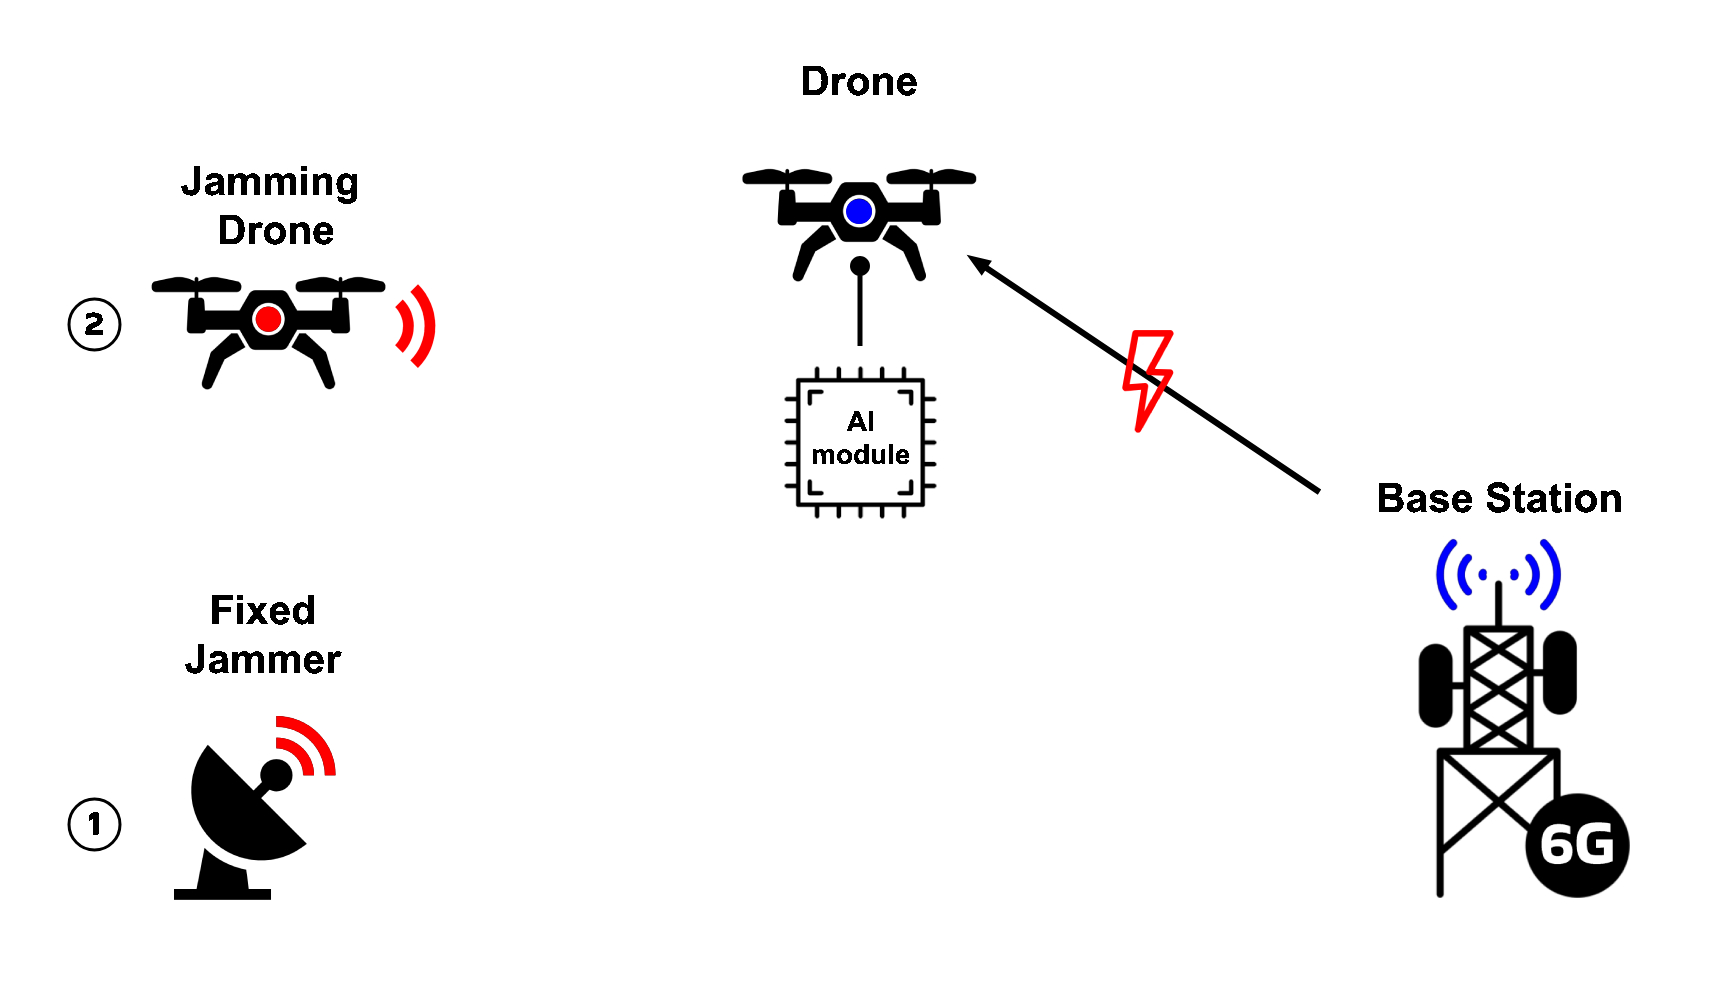
\includegraphics[width=10.5 cm]{img/CombinedJammingscenariosDiagram.jpg}
	\centering
	\caption{Proposed jamming scenario. The Drone communicates with the 6G BS and receives information about how to behave. The fixed jammer \textbf{(1)} and the mobile jammer \textbf{(2)} target the communication between the drone and the Base Station. The drone has an internal classification module capable of detecting jamming attacks.}
	\label{fig:CombinedJammingscenariosDiagram}
	\end{figure}   


In our scenario, the drone is subject to two types of jamming attacks, a constant and a periodic jamming attack that can be attributed to two different types of jammers. The constant jamming attack could be caused by a fixed ground jammer, as maintaining a constant jamming signal requires a large power source, while 
the periodic jamming attack could be caused by a mobile jammer, for example a drone, as drones are usually battery powered and can only jam for a limited amount of time. 
Employing a periodic jamming attack allows the malicious drone to preserve energy and lowers the chances of detection.

The attacker classification \cite{MLMisbehavior5GBoualouache} of the proposed scenario is detailed in Table \ref{tab:attacker_classification}: 

\begin{table}[H]
	\caption{Attacker classification details.\label{tab:attacker_classification}}
	\newcolumntype{C}{>{\centering\arraybackslash}X}
	\begin{tabularx}{\textwidth}{CC}
	\toprule
	\textbf{Classification} & \textbf{Description} \\
	\midrule
	Active   & The attacker is actively trying to disrupt network operation by transmitting a jamming signal\\
	External & The attack takes place at level 1 of the OSI model, meaning that the attacker is not part of the network\\
	Local    & The attack is local, as it is targeted at a specific drone or drone cluster and not at the entire network\\
	Malicious & Jamming attacks are considered malicious as their main goal is to disrupt correct network operation\\
	\bottomrule
\end{tabularx}
\end{table}

\subsection{Dataset Choice}\label{sec:DatasetChoice}

As 6G network traffic is not yet widely available, we chose an open-source dataset \cite{JammingDetectionIoT-Hussain} that analyses the RSS values 
received by a Raspberry Pi 3 which is subject to periodic and constant jamming attacks. 

The dataset in \cite{JammingDetectionIoT-Hussain} was created using a software-defined radio (SDR) connected to a laptop that was programmed to transmit a jamming signal using the 
open-source software \textit{GNU Radio}. A second SDR radio was connected to a Raspberry Pi 3, designated to receive the jamming signal. The jamming radio operates at a frequency of $2.412 GHz$ with a bandwidth of $40MHz$, while the Raspberry Pi 3 was programmed to sample the RSS values with a frequency of $32K$ samples per second. 

The dataset contains three different \textit{.txt} files that store the RSS values sampled by the Raspberry Pi 3. The first file contains the RSS values sampled during a constant jamming attack, the second file contains the RSS values sampled during a periodic jamming attack and the third file contains the RSS values sampled during normal network operation.
The samples are stored in a single column, with each row representing a single sampled RSS value, expressed in \textit{dBm (decibel-milliwatts)}. 

Figures \ref{fig:ConstantJammingSignal} and \ref{fig:PeriodicJammingSignal} show, respectively, plots of the RSS values sampled during a constant jamming attack and a periodic jamming attack, while Figure \ref{fig:normalSignal} shows the RSS values sampled during normal network operation.

\begin{figure}[H]
	\begin{adjustwidth}{-\extralength}{0cm}
	\centering
	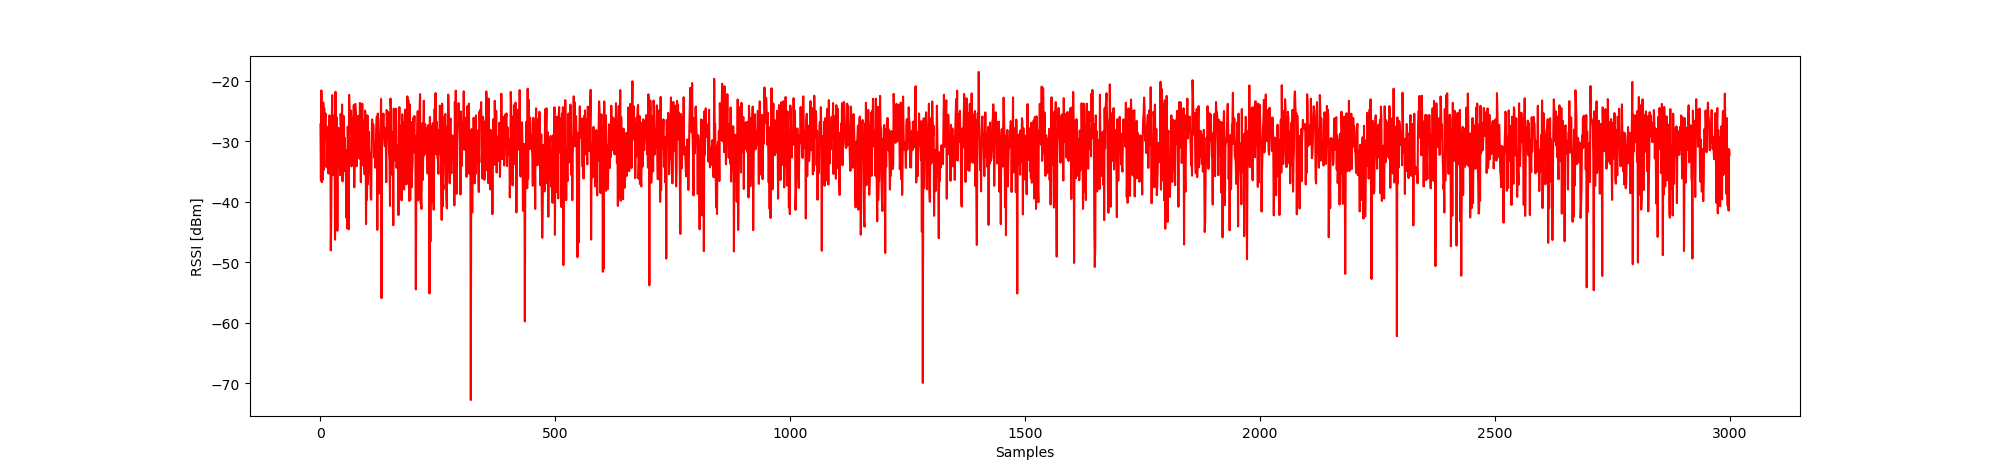
\includegraphics[width=21cm]{img/ConstantJammingSignal.png}
	\end{adjustwidth}
	\caption{Constant jamming attack RSS values}\label{fig:ConstantJammingSignal}
\end{figure}  
\unskip
\begin{figure}[H]
	\begin{adjustwidth}{-\extralength}{0cm}
	\centering
	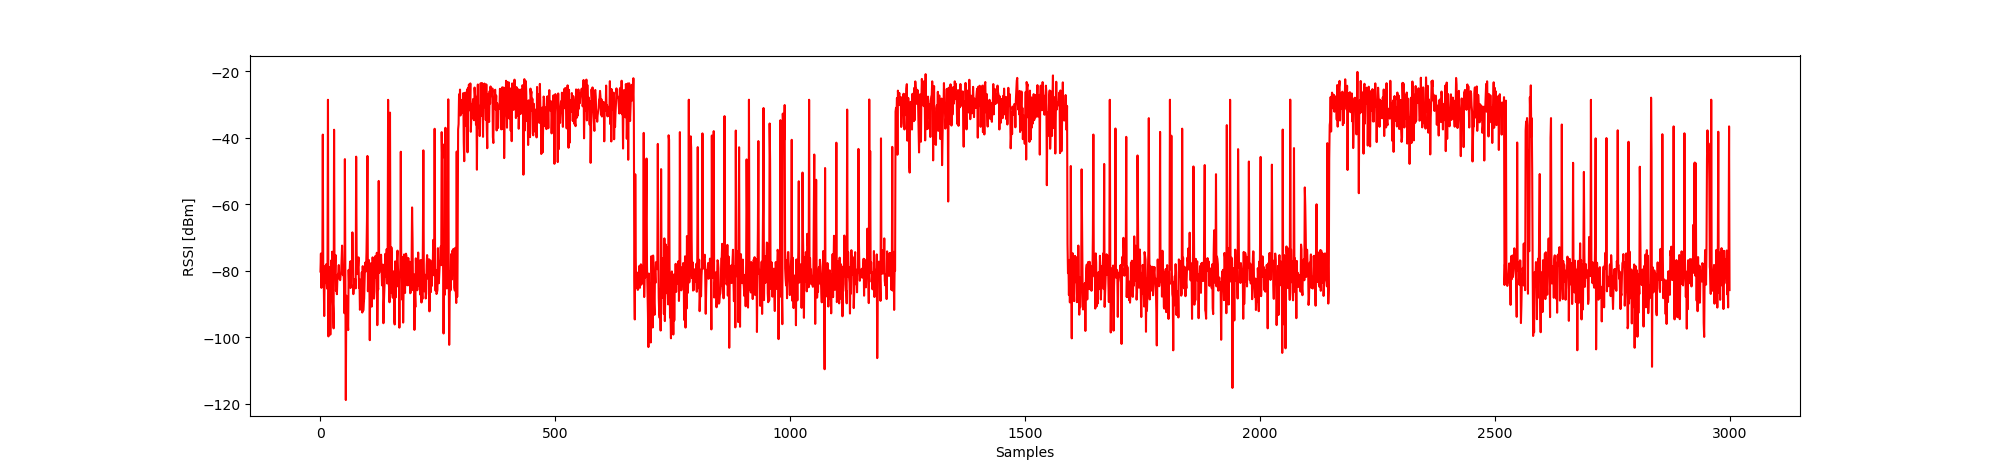
\includegraphics[width=21cm]{img/PeriodicJammingSignal.png}
	\end{adjustwidth}
	\caption{Periodic jamming attack RSS values}\label{fig:PeriodicJammingSignal}
\end{figure}  
\unskip

\begin{figure} [H]
	\begin{adjustwidth}{-\extralength}{0cm}
	\centering
	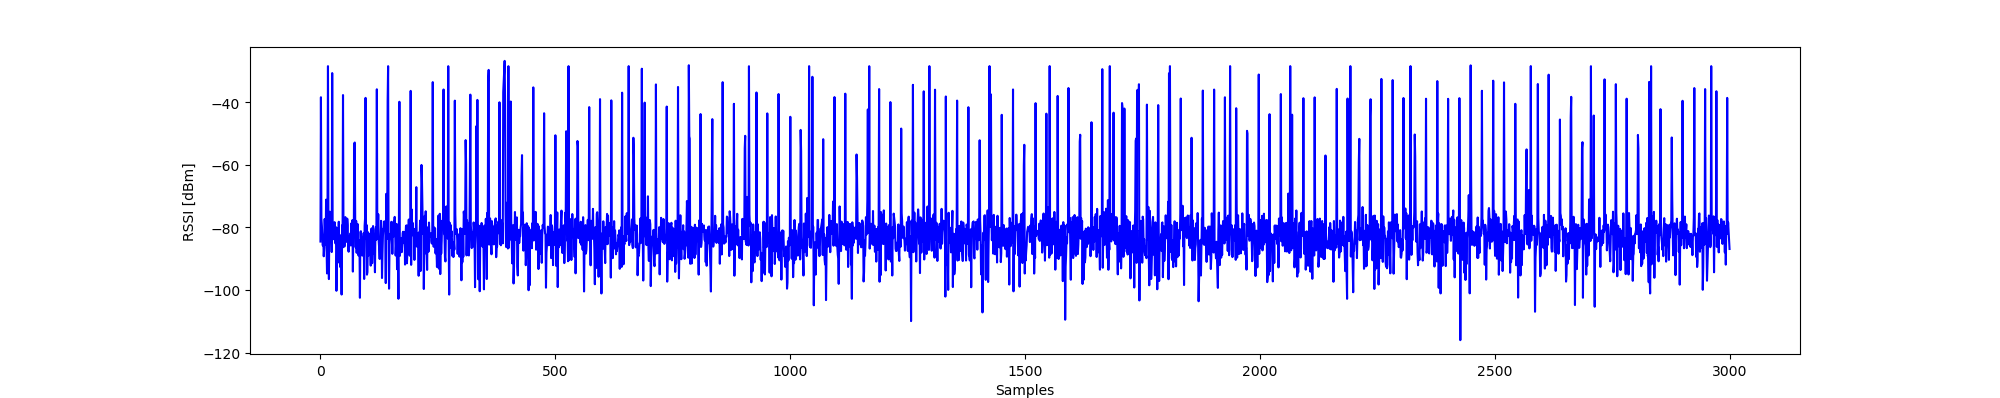
\includegraphics[width=21cm]{img/NormalSignal.png}
	\end{adjustwidth}
	\caption{Normal network operation RSS values}\label{fig:normalSignal}
\end{figure}
\unskip

\subsection {Detection Algorithm}

When choosing the algorithm for the classification module, we first had to define the requirements that it has to meet. The algorithm has to have the ability to classify anomalous samples with a high detection rate (Recall), while at the same time 
being lightweight enough in terms of memory usage and computational power to be run on a resource-constrained device like a drone. The training phase should also be fast, as this would allow the drone to quickly determine the normal transmission RSS values in a constantly changing environment. A periodic redefinition of normal RSS values would 
limit the number of false positives caused by drone mobility. 
The model should also require a small amount of storage to run effectively, as drones are usually very limited in internal memory. 

The algorithm that we found to be the best fit for these requirements is the \textit{Isolation Forest} algorithm \cite{IsolationForestLiu}. The Isolation Forest (IF) algorithm is a state-of-the-art unsupervised ML algorithm for anomaly detection, introduced by Liu et al. in 2008. 
Unlike traditional anomaly detection algorithms, which require the definition of a normal class, IF is able to detect anomalies without explicitly defining their characteristics.
This is achieved by leveraging the properties of anomalies themselves, i.e., being rare and separated from the majority of the data points. 

The algorithm works by building a forest of isolation trees. Each tree is built by randomly selecting one of the features and then splitting the data points based on a value randomly selected between the minimum and maximum value of the feature. This partitions the data into the 
left and right branches of the tree. The process is repeated recursively until all the data points are isolated. The height of a node, meaning the number of splits required to isolate it, is used to determine the anomaly score of the data point. The greater the number of splits, the more likely the data point is to be an anomaly.
IF is an \textit{ensemble} algorithm, meaning that the final anomaly score is calculated by averaging the anomaly scores of all the trees in the forest. More trees result in greater accuracy but also more computational power required.

The algorithm was chosen for its simplicity, low computational requirements (both in terms of memory and computational power) and proven effectiveness in the detection of anomalies\cite{IsolationForestLiu}. While more complex solutions like Neural Networks or Support Vector Machines might prove more effective in certain scenarios, they are best suited in a situation where computation power is not a limiting factor.
The unsupervised nature of the algorithm was also a determining factor in its selection, as it would allow for a periodical redefinition of the normal RSS values based on the current environment, without the need to rely on a fixed labeled dataset. 
Also, thanks to the ability to work on high dimensional data, the algorithm could potentially be scaled to work with more complex datasets in the future, if the drones were to be equipped with more advanced sensors.

The chosen implementation for IF is the one provided by the \textit{Scikit-learn} library \cite{IsolationForestScikitLearn} for Python 3. The model was tested on both a Raspberry Pi 3 and a desktop processor, demonstrating effective performance in both environments with comparable trends. The presented graphs reflect results from the desktop processor, but the model's efficiency on resource-constrained devices has been validated.

\subsection{Evaluation Metrics}\label{EvaluationMetrics}

The performance of the model was evaluated using the state-of-the-art evaluation metrics for ML classification algorithms. The metrics are all based on the number of true positives, false positives, true negatives and false negatives.
The chosen evaluation metrics are the following: 

\begin{itemize}
	\item \textbf{Accuracy:} the ratio of correctly classified data points to the total number of data points.
	\begin{equation}
		\label{eq:accuracy}
	  Accuracy = \frac{TP + TN}{TP + TN + FP + FN}
	\end{equation}
	\item \textbf{Precision:} the ratio of correctly classified anomalies to the total number of data points classified as anomalies.
	\begin{equation}
		\label{eq:precision}
	  Precision = \frac{TP}{TP + FP}
	\end{equation}
	\item \textbf{Recall:} the ratio of correctly classified anomalies to the total number of anomalies.
	\begin{equation}
		\label{eq:recall}
	  Recall = \frac{TP}{TP + FN}
	\end{equation}
	\item \textbf{F1 Score:} the harmonic mean of the precision and recall.
	\begin{equation}
		\label{eq:f1}
	  F1 = 2 \times \frac{Precision \times Recall}{Precision + Recall}
	\end{equation}
\end{itemize}
The combination of these metrics gives us concrete insight into the performance of the model. 

%%%%%%%%%%%%%%%%%%%%%%%%%%%%%%%%%%%%%%%%
\section{Model Performance }

\subsection{Parameters Tuning Phase}

The first phase in our testing methodology involves tuning the model's hyperparameters by varying them between a minimum and a maximum value, evaluating the impact on the performance metrics (detailed in Section \ref{EvaluationMetrics}) and then choosing the best possible values. 
In our scenario, a value is considered good if it provides a high metric value while at the same time not impacting too drastically the execution time. In cases where improving the value of a metric requires a significant increase in execution time, we chose the value that provides the best trade-off between the two.

Among the parameters available in the \textit{Scikit-learn} implementation of the Isolation Forest, we decided to tune the following: 

\begin{itemize}
	\item \textbf{n\_estimators:} the number of base estimators in the ensemble, i.e., the number of isolation trees used to compute the anomaly score of each data point. 
	\item \textbf{max\_samples:} the max number of samples to draw from the dataset to train each tree.
	\item \textbf{contamination:} the amount of outliers present in the training dataset.  
\end{itemize} 
During the tuning phase, the untested hyperparameters were set to the default values of the \textit{Scikit-learn} implementation of the Isolation Forest (Table \ref{tab:isolation_forest_parameters}).

\begin{table}[H]
	\caption{Scikit-Learn Isolation Forest hyperparameters default values.\label{tab:isolation_forest_parameters}}
	\newcolumntype{C}{>{\centering\arraybackslash}X}
	\begin{tabularx}{\textwidth}{CC}
	\toprule
	\textbf{Parameter} & \textbf{Default Value} \\
	\midrule
	n\_estimators & 100 \\
	max\_samples & 'auto' \\
	contamination & 0.1 \\
	\bottomrule
	\end{tabularx}
\end{table}

The model was evaluated using input composed of normal traffic samples concatenated with jamming attack samples (see code snippet \ref{alg:dataset_concatenation}). 
This was done to simulate a real-world scenario where the model has to be able to correctly classify anomalous samples but also reduce the number of false positives during normal operation. 

\begin{algorithm}
	\caption{Test input definition}\label{alg:dataset_concatenation}
	\begin{algorithmic}[1]
	\State normalTraffic $\gets$ ReadAndParseFile(NORMAL\_TRAFFIC\_FILE, normal\_traffic\_size)
	\State jamming $\gets$ ReadAndParseFile(JAMMING\_FILE, jamming\_size)

	\State testInput $\gets$ Concatenate(normalTraffic, jamming)
	\end{algorithmic}
\end{algorithm}

The selected values for \textit{normal\_traffic\_size} and \textit{jamming\_size} are shown in Table \ref{tab:dataset_sizes}. 

\begin{table}[H]
	\caption{Dataset sizes used for the tuning and testing phases.}\label{tab:dataset_sizes}
	\newcolumntype{C}{>{\centering\arraybackslash}X}
	\begin{tabularx}{\textwidth}{CC}
	\toprule
	\textbf{Dataset} & \textbf{Size} \\
	\midrule
	normal\_traffic\_size & 20,000 \\
	jamming\_size & 2,000 \\
	\bottomrule
\end{tabularx}
\end{table}

The dataset is intentionally unbalanced between normal data points and anomalous points, as jamming attacks are usually rare events compared to normal network operation. 
In Figure \ref{fig:InputSignal} we can see a representation of the input signal in the case of a constant jamming attack. The proposed results, unless otherwise specified, are based on the input signal shown in Figure \ref{fig:InputSignal}, which employs constant jamming. Periodic jamming has always shown comparable trends as constant jamming in all the performed tests.


\begin{figure}[H]
    \begin{adjustwidth}{-\extralength}{0cm}
        \centering
        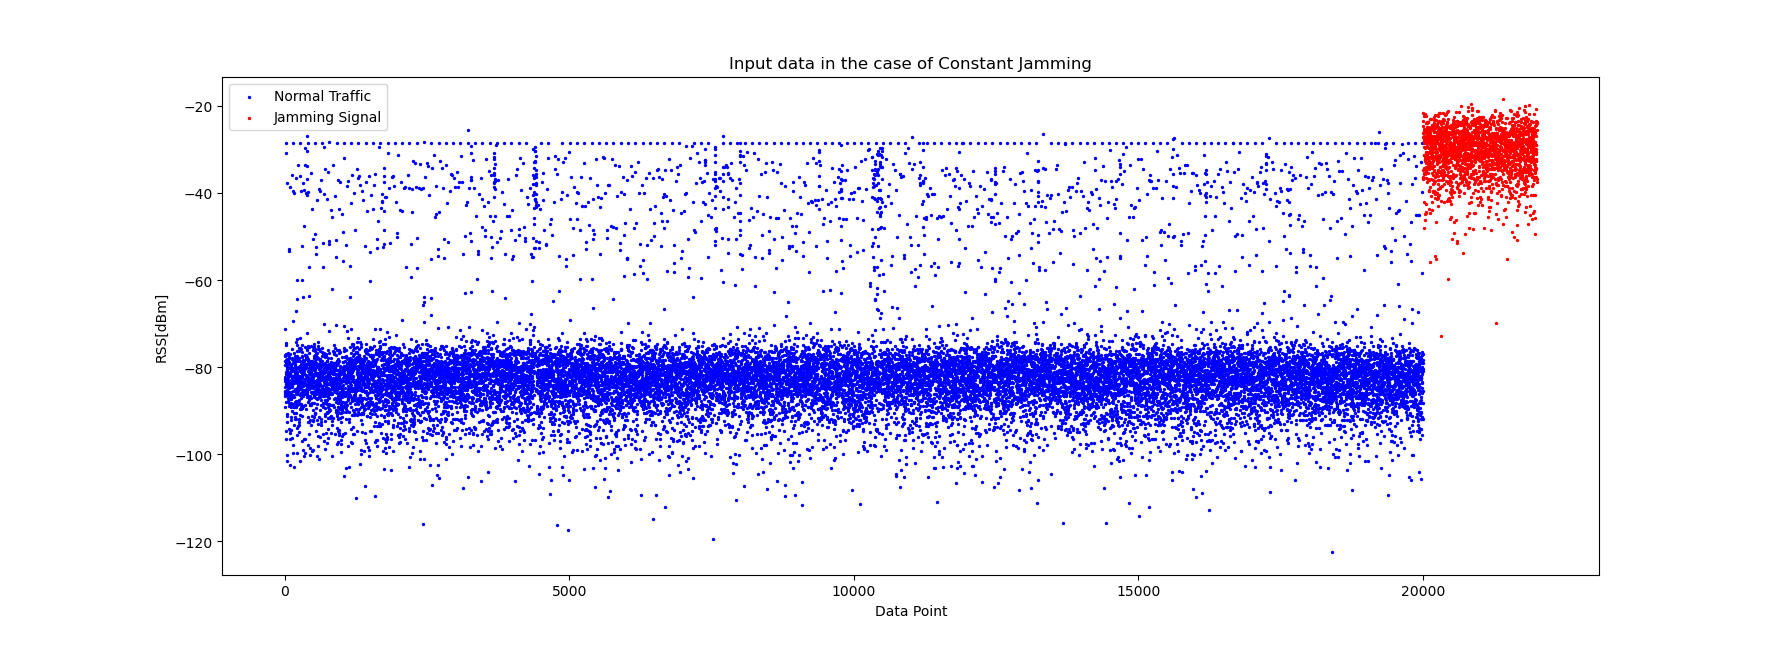
\includegraphics[width=21cm]{img/InputSignal.png}
    \end{adjustwidth}
    \caption{Input signal in the case of Constant jamming. The normal traffic signal is concatenated with the jamming signal.}
    \label{fig:InputSignal}
\end{figure}


\subsubsection{n\_estimators tuning}

The first parameter that we decided to tune was the \textit{n\_estimators} parameter. The tuning values are shown in Table \ref{tab:n_estimators_tuning}.

\begin{table}[H]
	\caption{n\_estimators tuning values.}\label{tab:n_estimators_tuning}
	\newcolumntype{C}{>{\centering\arraybackslash}X}
	\begin{tabularx}{\textwidth}{CC}
	\toprule
	\textbf{n\_estimators} & \textbf{Values} \\
	\midrule
	Minimum & 1 \\
	Maximum & 50 \\
	Step & 1 \\
	\bottomrule
\end{tabularx}
\end{table}

The effect on the evaluation metrics of the model is shown in Figure \ref{fig:n_estimators_tuning}.

\begin{figure}[H]
	\centering
	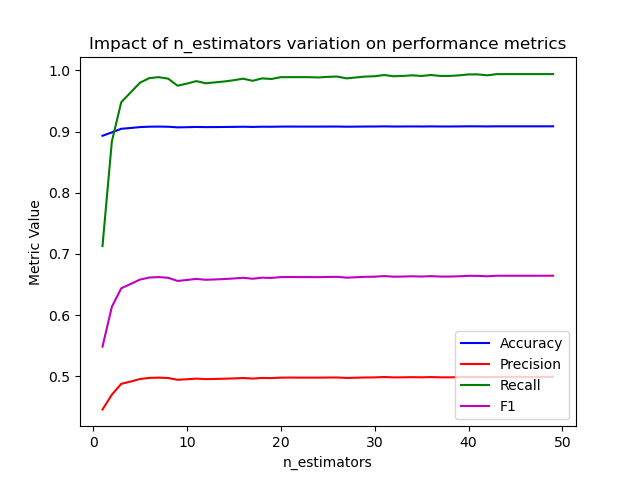
\includegraphics[width=10.5cm]{img/nEstimatorsTuning.png}
	\caption{n\_estimators tuning results. Performance of the model in all analyzed metrics increases with an increasing number of estimators}\label{fig:n_estimators_tuning}
\end{figure}
\unskip

As we can see from the graph, performance increases as the number of estimators increase, converging to a stable value. 
Graphs \ref{fig:n_estimators_training_time} and \ref{fig:n_estimators_classification_time} show that the time required both for training and classification increases linearly with the number of estimators.
This means that choosing an appropriate number of estimators is crucial, as it can greatly affect the model performance. 

\begin{figure}[H]
    \centering
    \begin{subfigure}{0.49\textwidth}
        \centering
        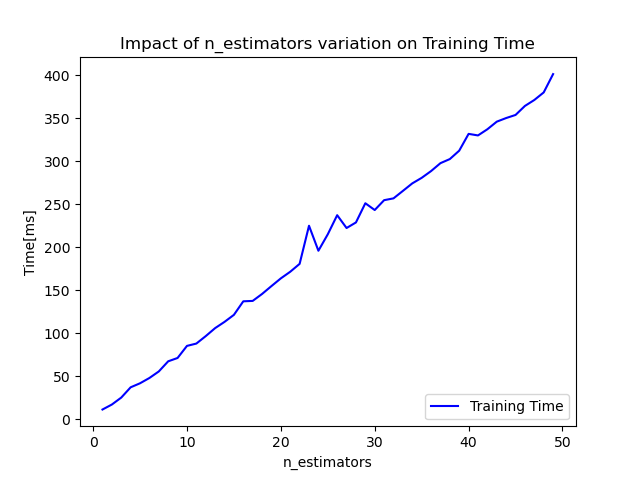
\includegraphics[width=\textwidth]{img/nEstimatorsTrainingTime.png}
        \caption{n\_estimators training time.}
        \label{fig:n_estimators_training_time}
    \end{subfigure}
    \hfill
    \begin{subfigure}{0.49\textwidth}
        \centering
        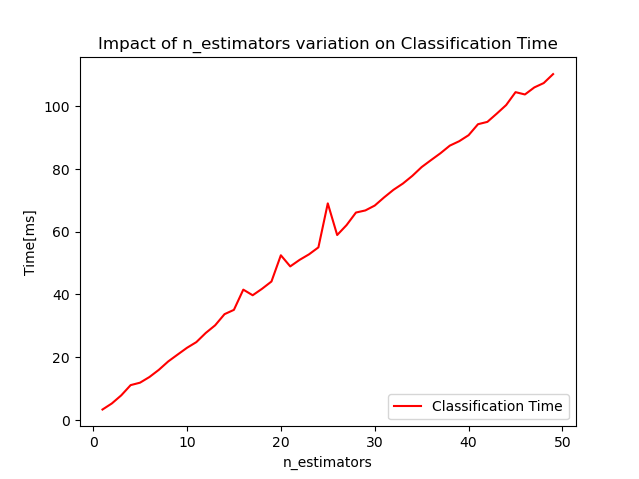
\includegraphics[width=\textwidth]{img/nEstimatorsClassificationTime.png}
        \caption{n\_estimators classification time.}
        \label{fig:n_estimators_classification_time}
    \end{subfigure}
    \caption{Comparison of n\_estimators training and classification times. Both training and classification times increase linearly with the number of estimators.}
    \label{fig:estimators_time_comparison}
\end{figure}


We accordingly selected \textbf{n\_estimators = 15}, as it provided a good balance between model performance and computational resources required.
The model metrics keep slowly improving until $45$ estimators, but the performance increase is minimal, making it not worth such a large increase in training and classification time, especially considering the resource-constrained nature of the scenario under consideration. 

\subsubsection{max\_samples tuning}

The second parameter that we decided to tune was the \textit{max\_samples} parameter. The tuning values are shown in Table \ref{tab:max_samples_tuning}.

\begin{table}[H]
	\caption{max\_samples tuning values.}\label{tab:max_samples_tuning}
	\begin{tabularx}{\textwidth}{CC}
	\toprule
	\textbf{max\_samples} & \textbf{Values} \\
	\midrule
	Minimum & 1 \\
	Maximum & 100 \\
	Step & 1 \\
	\bottomrule
\end{tabularx}
\end{table}

From Figure \ref{fig:max_samples_tuning} we can notice that the model performance is not greatly affected by the \textit{max\_samples} parameter. This is most likely due to the significant difference in RSS values between the normal traffic samples and the jamming attack samples, meaning the model can develop the ability to correctly classify the input even with a limited training set.

\begin{figure}[H]
	\centering
	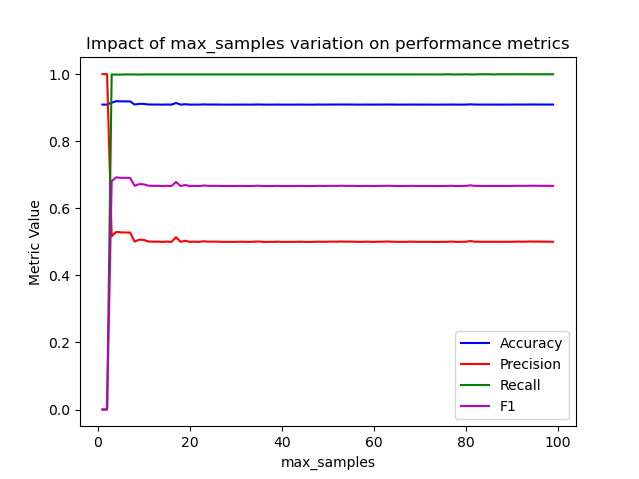
\includegraphics[width=10.5cm]{img/maxSamplesTuning.png}
	\caption{max\_samples tuning results. The max samples parameter has limited impact on the model's performance given the large difference in RSS values between normal and anomalous samples.}\label{fig:max_samples_tuning}
\end{figure}
\unskip

However, as the model has to build bigger trees, the \textit{max\_samples} parameter has considerable influence on the training and classification time, as shown in Figure \ref{fig:max_samples_time_comparison}.
Given the minimal performance differences but substantial impact on the time metrics, we chose the value of \textbf{max\_samples = 10}. 

\begin{figure}[H]
	\centering
	\begin{subfigure}{0.49\textwidth}
		\centering
		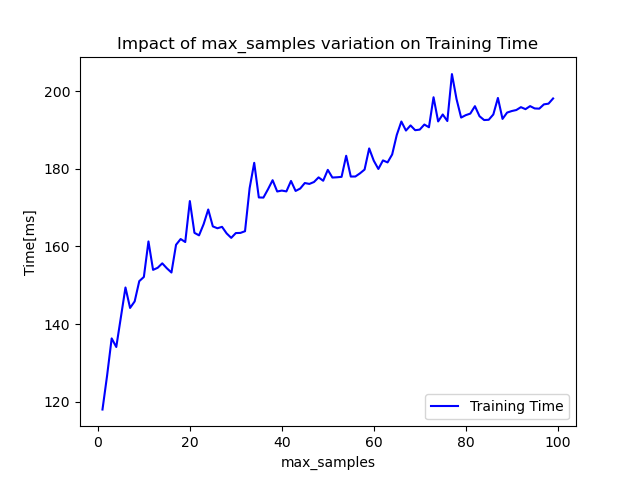
\includegraphics[width=\textwidth]{img/maxSamplesTrainingTime.png}
		\caption{max\_samples training time.}
		\label{fig:max_samples_training_time}
	\end{subfigure}
	\hfill
	\begin{subfigure}{0.49\textwidth}
		\centering
		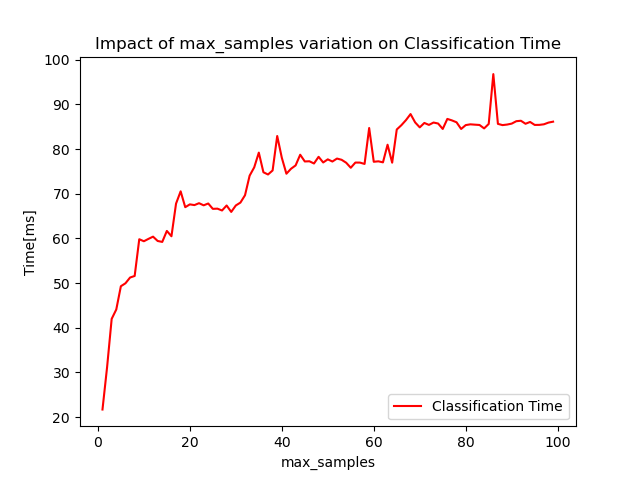
\includegraphics[width=\textwidth]{img/maxSamplesClassificationTime.png}
		\caption{max\_samples classification time.}
		\label{fig:max_samples_classification_time}
	\end{subfigure}
	\caption{Comparison of max\_samples training and classification times. Both training and classification times follow a logarithmic trend.}
	\label{fig:max_samples_time_comparison}
\end{figure}

\subsubsection{contamination tuning}

The last parameter we focused on is the \textit{contamination} parameter. The tuning values are shown in Table \ref{tab:contamination_tuning}.

\begin{table}[H]
	\caption{contamination tuning values.}\label{tab:contamination_tuning}
	\begin{tabularx}{\textwidth}{CC}
	\toprule
	\textbf{contamination} & \textbf{Values} \\
	\midrule
	Minimum & 0.01 \\
	Maximum & 0.5 \\
	Step & 0.01 \\
	\bottomrule
	\end{tabularx}
\end{table}

The contamination parameter is by far the one that has the greatest impact on the model performance, as shown in Figure \ref{fig:contamination_tuning}.
Since recall is the metric that we want to prioritize as it highlights the number of detections, we chose the value of \textbf{contamination = 0.09}.

\begin{figure}[H]
	\centering
	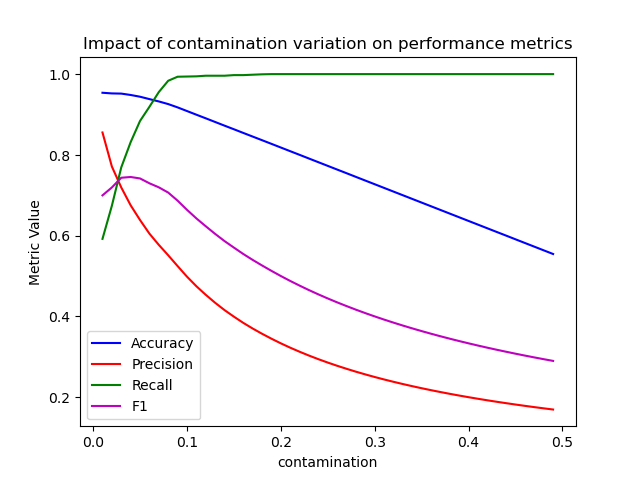
\includegraphics[width=10.5cm]{img/contaminationTuning.png}
	\caption{contamination tuning results. While recall score benefits from a higher contamination, all the other metrics are negatively impacted by a higher contamination value.}\label{fig:contamination_tuning}
\end{figure}
\unskip

Our testing pointed out that, as expected, tuning of the contamination parameter has minimal impact on the training and classification time. 

\subsection{Model Testing Phase}

\subsubsection{Standard Model Testing}\label{sec:standardModelTesting}

After the tuning phase, we tested the model using the best performing hyperparameters, detailed in Table \ref{tab:best_hyperparameters} and compared against the default parameters. 


\begin{table}[H]
	\caption{Tuned hyperparameters and default values} \label{tab:best_hyperparameters}
	\newcolumntype{C}{>{\centering\arraybackslash}X}
	\begin{tabularx}{\textwidth}{CCC}
	\toprule
	\textbf{Parameter} & \textbf{Tuned Value} & \textbf{Default Value} \\
	\midrule
	n\_estimators & 15 & 100 \\
	max\_samples & 10 & 'auto' \\
	contamination & 0.09 & 0.1 \\
	\bottomrule
	\end{tabularx}
\end{table}



The model was tested against the input signal shown in Figure \ref{fig:InputSignal}. In Figure \ref{fig:standardIsolationResults} we can see the results of the model classification of the input signal with the tuned hyperparameters. 

\begin{figure}[H]
	\begin{adjustwidth}{-\extralength}{0cm}
	\centering
	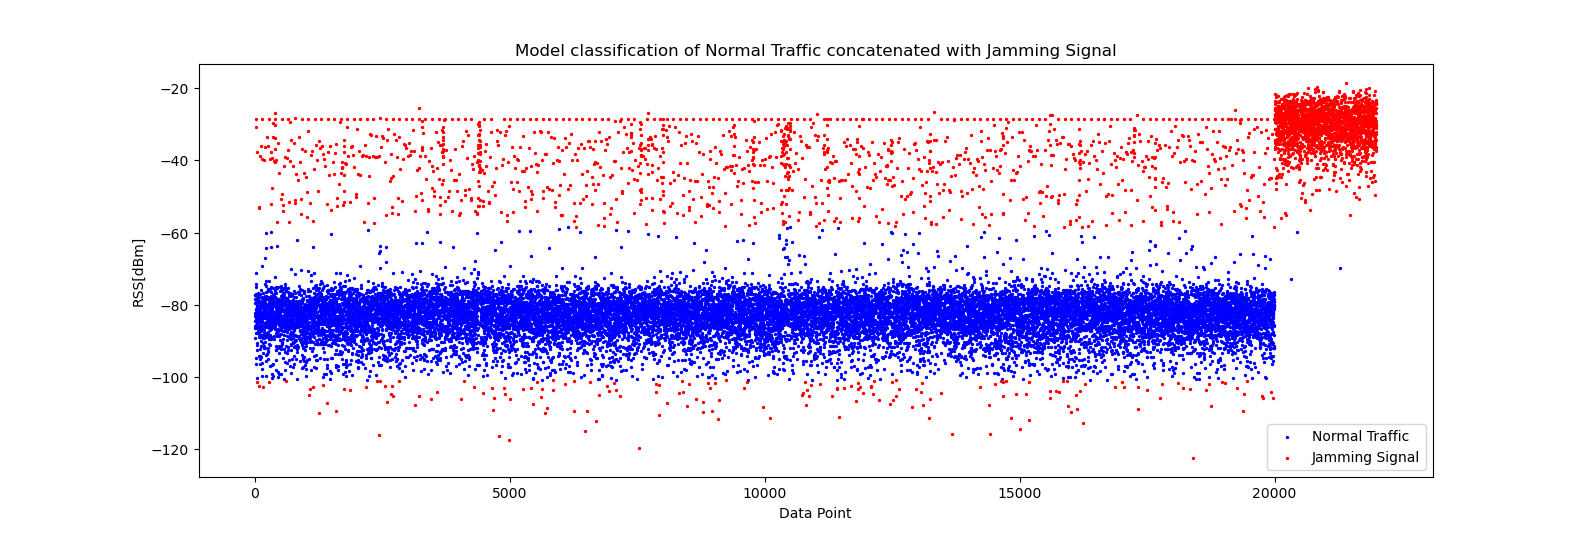
\includegraphics[width=21cm]{img/StandardIsolationForestClassification.png}
	\end{adjustwidth}
	\caption{Classification results from the tuned Isolation Forest model.}\label{fig:standardIsolationResults}
\end{figure}  

Table \ref{tab:confusionMatrix} and \ref{tab:performanceMetrics} show a comparison between the model performance with the tuned and the default hyperparameters.

\begin{table}[H]
    \caption{Confusion Matrix Components Comparison.}\label{tab:confusionMatrix}
    \newcolumntype{C}{>{\centering\arraybackslash}X}
    \begin{tabularx}{\textwidth}{CCC}
    \toprule
    \textbf{Metric} & \textbf{Tuned Isolation Forest} & \textbf{Default Isolation Forest} \\
    \midrule
    \textbf{TP} & 1997 & 2000 \\
    \textbf{FP} & 1565 & 1993 \\
    \textbf{TN} & 18435 & 18007 \\
    \textbf{FN} & 3 & 0 \\
    \bottomrule
    \end{tabularx}
\end{table}

Figures \ref{fig:ConfusionMatrixStandardIF} and \ref{fig:ConfusionMatrixTunedIF} show, respectively, the confusion matrix for the default and the tuned Isolation Forest model.

\begin{figure}[H]
	\centering
	\begin{subfigure}{0.49\textwidth}
		\centering
		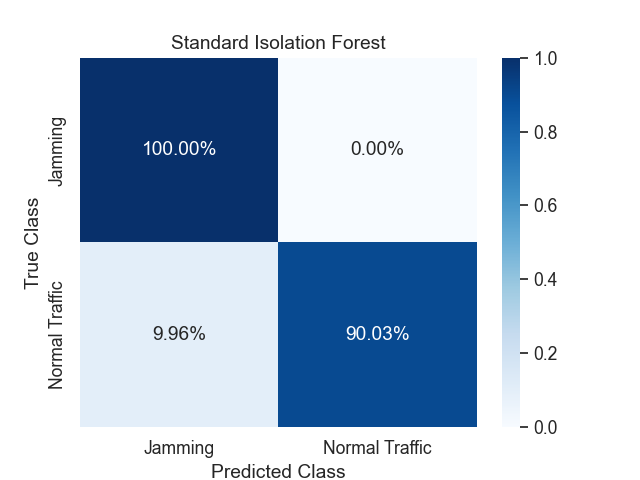
\includegraphics[width=\textwidth]{img/ConfusionMatrixStandardIF.png}
		\caption{}
		\label{fig:ConfusionMatrixStandardIF}
	\end{subfigure}
	\hfill
	\begin{subfigure}{0.49\textwidth}
		\centering
		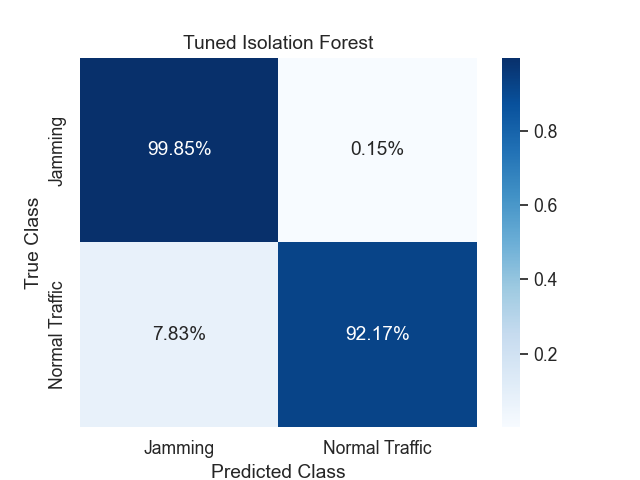
\includegraphics[width=\textwidth]{img/ConfusionMatrixTunedIF.png}
		\caption{}
		\label{fig:ConfusionMatrixTunedIF}
	\end{subfigure}
	\caption{Confusion Matrix for the default Isolation Forest model \textbf{(a)} and the tuned Isolation Forest model \textbf{(b)}. The tuned version reduces false positives while suffering a negligible increase in false negatives compared to the default model.}
	\label{fig:ConfusionMatrixStandardTunedIF}
\end{figure}


\begin{table}[H]
    \caption{Performance Metrics Comparison.}\label{tab:performanceMetrics}
    \newcolumntype{C}{>{\centering\arraybackslash}X}
    \begin{tabularx}{\textwidth}{CCC}
    \toprule
    \textbf{Metric} & \textbf{Tuned Isolation Forest} & \textbf{Default Isolation Forest} \\
    \midrule
    \textbf{Accuracy} & 0.929 & 0.909 \\
    \textbf{Precision} & 0.561 & 0.501 \\
    \textbf{Recall} & 0.999 & 1.000 \\
    \textbf{F1 Score} & 0.718 & 0.667 \\
    \bottomrule
    \end{tabularx}
\end{table}


The tuning phase proved effective in improving the model's performance compared to the default hyperparameters, with an increase of $2\%$ in accuracy, $6\%$ in precision, and $5.1\%$ in the F1 score, while maintaining a nearly identical recall ($0.1\%$ drop). However, despite reaching a very high Recall score in both scenarios, the model is still too prone to false positives, as indicated by the value of the Precision metric. 
This is most likely due to the nature of the normal traffic signal. As we see from Figure \ref{fig:standardIsolationResults}, many of the normal traffic samples have RSS values that are similar to the jamming attack samples, leading the model to classify them as anomalies.
This is most likely due to how the dataset has been created, as the normal traffic samples were measured in a real-world scenario where the RSS values would be affected by external noise. 

Instead of seeing this as an impairment, we view it as an improvement opportunity. The fact that the dataset contains noise means it is more representative of a real-world scenario, where the drone might be moving through different environments and thus be subject to environmental noise.

\subsubsection{Majority Rule model testing} \label{sec:majorityRuleModelTesting}

Having understood the nature of the problem, we decided to implement a Majority Rule (MR) system to reduce the number of false positives. The improved model would use the Tuned Isolation Forest model's results and then pass them to a MR module, as shown in Figure \ref{fig:MajorityRuleDiagram}. 

\begin{figure}[H]
	\centering
	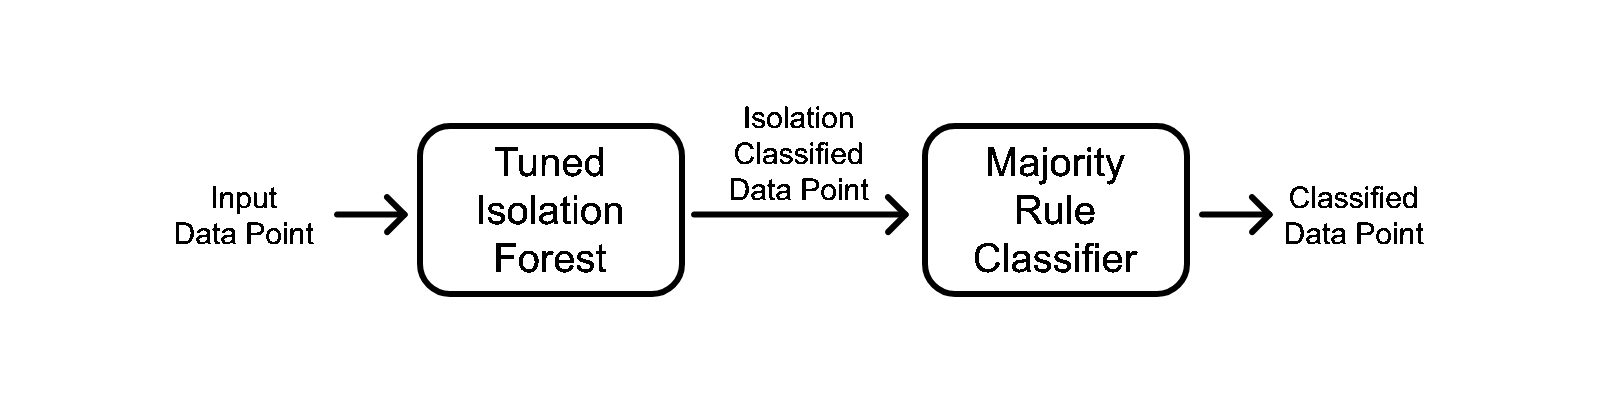
\includegraphics[width=12.5 cm]{img/ModulesStructure.jpg}
	\caption{Majority Rule system diagram. The Tuned Isolation Forest model results are passed to the MR module, which then provides the final classification.}
	\label{fig:MajorityRuleDiagram}
	\end{figure}   


The logic behind the Majority Rule module is simple. The MR takes as input the classification results of the IF model and inserts them into a sliding window. If the data point is classified by the Tuned IF as an anomaly, the MR module checks the contents of the sliding window. If the 
majority of the data points in the window are classified as anomalies, the data point is classified as an anomaly. If the majority of the data points in the window are classified as normal, then the data point is classified as normal (see code snipped \ref{alg:majority_rule}).

\begin{algorithm}
	\caption{Majority Rule Algorithm}\label{alg:majority_rule}
	\begin{algorithmic}[1]
		\State \hspace{1em} $\text{window} \leftarrow []$
		
		\For{each index in range(len(classification))}
			\If{length of window equals predefined window size}
				\State \hspace{1em} $\text{window.pop}(0)$
			\EndIf
			
			\State \hspace{1em} $\text{window.append}(\text{classification}[index])$
			
			\If{current classification is OUTLIER and the count of OUTLIERS in the window 
		 \State is less than or equal to half the window size}
				\State \hspace{1em} $\text{classification}[index] \leftarrow \text{INLIERS}$
			\EndIf
		\EndFor
		
		\State \hspace{1em} $\text{return classification}$
	\end{algorithmic}
\end{algorithm}

To determine the optimal value for the \textit{window\_size} parameter, we test the model in the same way as in the hyperparameters tuning phase. The model parameters were set to the best performing values from the tuning phase (Table \ref{tab:best_hyperparameters}). Table \ref{tab:window_size_tuning} shows the tuning values for the \textit{window\_size} parameter.

\begin{table}[H]
	\centering
	\caption{window\_size tuning values.}\label{tab:window_size_tuning}
	\begin{tabularx}{\textwidth}{CC}
	\toprule
	\textbf{window\_size} & \textbf{Values} \\
	\midrule
	Minimum & 1 \\
	Maximum & 100 \\
	Step & 1 \\
	\bottomrule
\end{tabularx}
\end{table}

From Figure \ref{fig:window_size_tuning} we can see that the \textit{window\_size} parameter has a considerable impact on the model performance. 
\begin{figure}[H]
	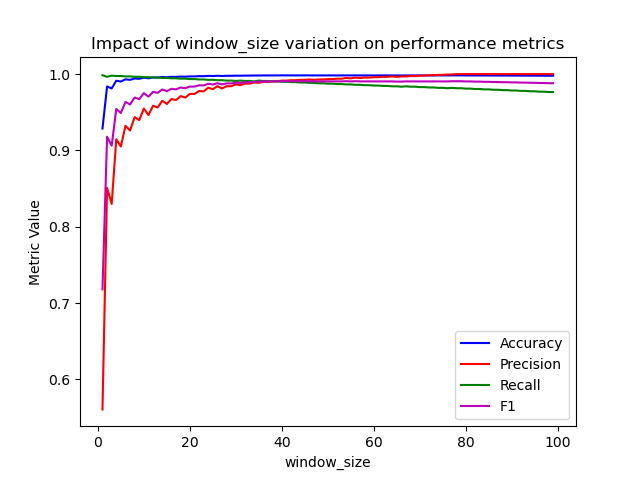
\includegraphics[width=10.5cm]{img/WindowSizeTuning.png}
	\caption{window\_size tuning results. Most metrics initially benefit from a larger window size except for recall that suffers a linear decrease.}\label{fig:window_size_tuning}
\end{figure}


While accuracy and precision benefit from a larger window size, we can observe a linear decrease in recall as the window size increases.
This is due to the nature of the majority rule, as a larger window size means that a larger number of anomalous data points must be present in the window in order to classify the current data point as an anomaly.
The optimal value for the \textit{window\_size} parameter was found to be \textbf{window\_size = 39}, as it provides high accuracy and precision while maintaining a high recall.

After defining the value for the \textit{window\_size} parameter, we tested the model against the same input signal used for the standard tuned model (Figure \ref{fig:InputSignal}). The results of the model classification are shown in Figure \ref{fig:majorityRuleIsolationResults}. 

\begin{figure}[H]
	\begin{adjustwidth}{-\extralength}{0cm}
	\centering
	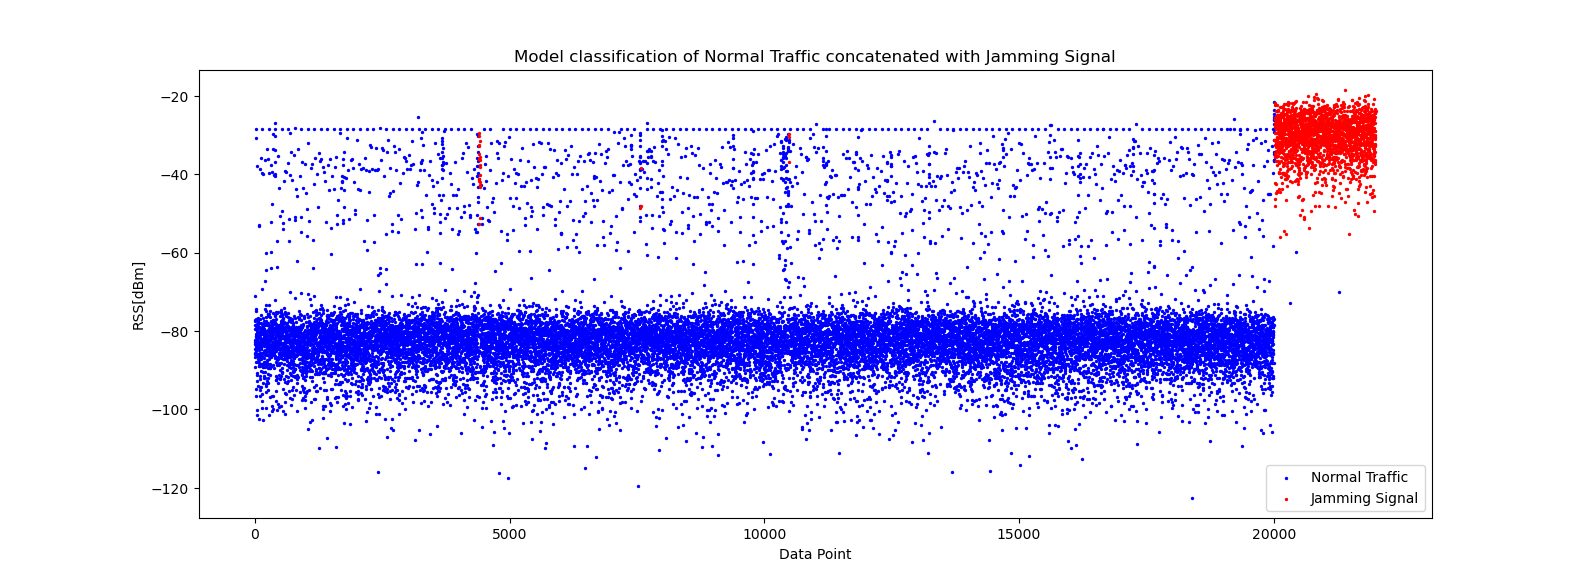
\includegraphics[width=21cm]{img/MajorityRuleIsolatioForestClassification.png}
	\caption{Classification results from the MR Isolation Forest model}\label{fig:majorityRuleIsolationResults}
	\end{adjustwidth}
\end{figure}

In Tables \ref{tab:majority_rule_confusionMatrix} and \ref{tab:majority_rule_performanceMetrics} we can see a comparison between the tuned model and the MR model.

\begin{table}[H]
    \caption{Confusion Matrix Components Comparison.}\label{tab:majority_rule_confusionMatrix}
    \begin{tabularx}{\textwidth}{CCC}
    \toprule
    \textbf{Metric} & \textbf{Tuned Isolation Forest} & \textbf{Majority Rule Isolation Forest} \\
    \midrule
    \textbf{TP}  & 1997  & 1982 \\
    \textbf{FN}  & 3     & 18   \\
    \textbf{FP}  & 1565  & 27   \\
    \textbf{TN}  & 18435 & 19973 \\
    \bottomrule
    \end{tabularx}
\end{table}

\begin{figure}[H]
	\centering
	\begin{subfigure}{0.49\textwidth}
		\centering
		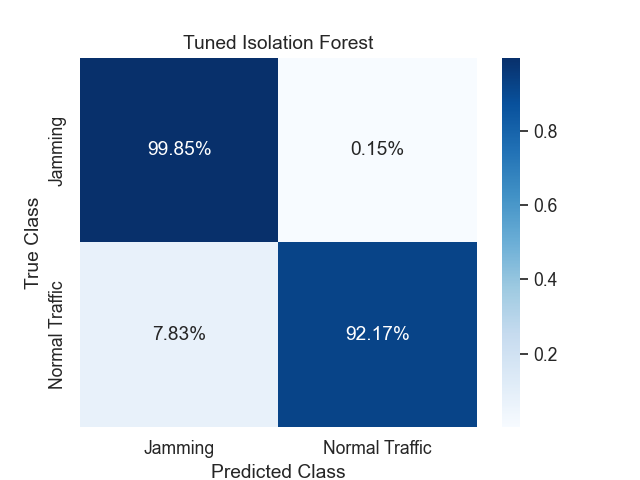
\includegraphics[width=\textwidth]{img/ConfusionMatrixTunedIF.png}
		\caption{}
		\label{fig:ConfusionMatrixStandardTunedIF1}
	\end{subfigure}
	\hfill
	\begin{subfigure}{0.49\textwidth}
		\centering
		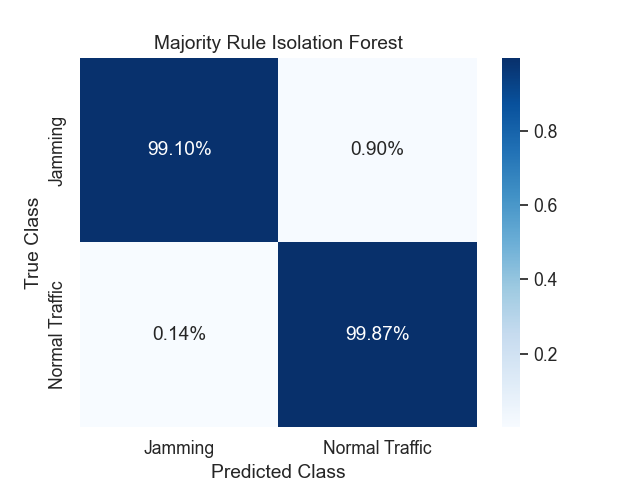
\includegraphics[width=\textwidth]{img/ConfusionMatrixMajorityIF.png}
		\caption{}
		\label{fig:ConfusionMatrixMajorityIF}
	\end{subfigure}
	\caption{Confusion Matrix for the tuned Isolation Forest model \textbf{(a)} and the Majority Rule Isolation Forest model \textbf{(b)}. The MR model significantly reduces false positives while maintaining a rate of true positives of over 99\%.}
	\label{fig:ConfusionMatrixTunedMajorityIF}
\end{figure}

\begin{table}[H]
    \caption{Performance Metrics Comparison.}\label{tab:majority_rule_performanceMetrics}
    \begin{tabularx}{\textwidth}{CCC}
    \toprule
    \textbf{Metric} & \textbf{Tuned Isolation Forest} & \textbf{Majority Rule Isolation Forest} \\
    \midrule
    \textbf{Accuracy}  & 0.929 & 0.998 \\
    \textbf{Precision} & 0.561 & 0.987 \\
    \textbf{Recall}    & 0.999 & 0.991 \\
    \textbf{F1 Score}  & 0.718 & 0.989 \\
    \bottomrule
    \end{tabularx}
\end{table}

The results show that the Majority Rule Model is effective in mitigating the high number of false positives that were present in the first version of the model. 
The MR integration resulted in an improvement in Precision of $42.6\%$, in Accuracy of $6.9\%$ and in F1 Score of $27.1\%$, while suffering only a less than $1\%$ drop in Recall.
In the original model, most of the false positives occurred due to the normal traffic samples containing a high number of isolated data points with similar RSS values to those of the jamming samples. 
The MR module addresses this by checking if the previous points were also classified as anomalies. This approach proves to be effective, as jamming attacks are rarely composed of isolated data points.

Given the resource-constrained nature of the scenario, we decided to test the computational impact of the MR module against the standard tuned model. 
Classification times and training times were measured for both models and the results are shown in Figures \ref{fig:majority_rule_classification_time} and \ref{fig:majority_rule_training_time}.

\begin{figure}[H]
	\centering
	\begin{subfigure}{0.49\textwidth}
		\centering
		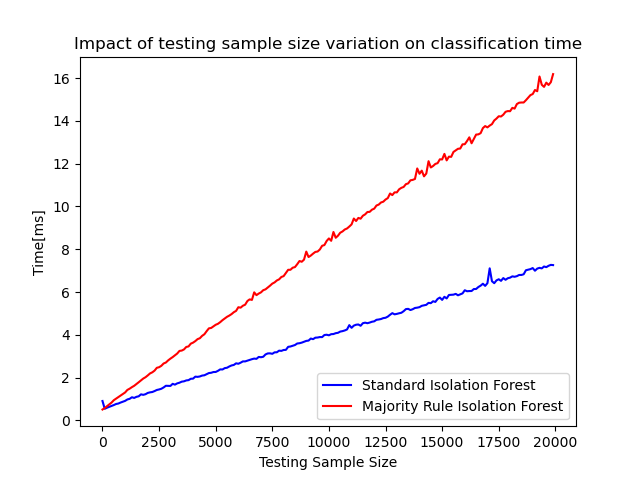
\includegraphics[width=\textwidth]{img/classificationTimeComparison.png}
		\caption{}
		\label{fig:majority_rule_classification_time}
	\end{subfigure}
	\hfill
	\begin{subfigure}{0.49\textwidth}
		\centering
		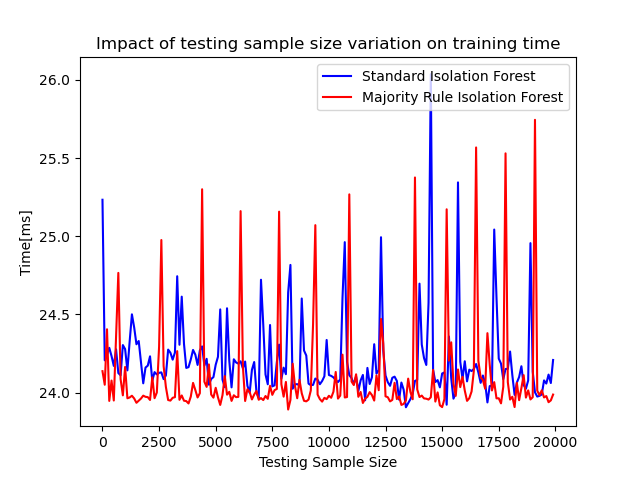
\includegraphics[width=\textwidth]{img/trainingTimeComparison.png}
		\caption{}
		\label{fig:majority_rule_training_time}
	\end{subfigure}
	\caption{Comparison of the standard tuned model and the MR in terms of classification time \textbf{(a)} and training time \textbf{(b)}.}
	\label{fig:majority_rule_time_comparison}
\end{figure}

Figure \ref{fig:majority_rule_classification_time} shows that there is indeed a difference in classification time, with the standard model being faster. This is due to the additional computational complexity added by the Majority Rule module, which requires updating and checking of the sliding window for each classified data point. 
Figure \ref{fig:majority_rule_training_time} on the other hand shows that, as expected, training time is not affected by the MR module.

\subsubsection{Comparison against existing solution}\label{sec:comparisonAgainstExistingSolution}

As mentioned in Section \ref{sec:DatasetChoice}, this work is based on the work of \cite{JammingDetectionIoT-Hussain}, where the authors proposed a solution for jamming attack detection based on CNNs. In their paper, one of the drawbacks that the authors cite with their solution is the low detection rate against periodic jamming, as well as an unreliable classification of normal traffic. 
We decided to compare our solution against the solution of the authors of the dataset we used. 
The results show two significant Figures as the results provided in the compared paper were in this format. Results in the case of constant jamming were very similar, with both models scoring $1.0$ in all the metrics and are therefore not shown.

Table \ref{tab:periodic_jamming_comparison} shows the comparison between the two models in the case of periodic jamming and Table \ref{tab:normal_traffic_comparison} shows the comparison between the two models in classification of normal traffic.


\begin{table}[H]
	\caption{Comparison between the proposed approach and the approach of \cite{JammingDetectionIoT-Hussain} in the case of periodic jamming.}\label{tab:periodic_jamming_comparison}
	\newcolumntype{C}{>{\centering\arraybackslash}X}
	\begin{tabularx}{\textwidth}{CCC}
	\toprule
	\textbf{Metric} & \textbf{Proposed Approach} & \textbf{CNN Approach} \\
	\midrule
	\textbf{Accuracy}  & 0.98 & 0.72 \\
	\textbf{Precision} & 0.99 & 0.73 \\
	\textbf{Recall}    & 0.95 & 0.83 \\
	\textbf{F1 Score}  & 0.97 & 0.78 \\
	\bottomrule
	\end{tabularx}
\end{table}

\begin{table}[H]
	\caption{Comparison between the proposed approach and the approach of \cite{JammingDetectionIoT-Hussain} in the case of normal traffic classification.}\label{tab:normal_traffic_comparison}
	\newcolumntype{C}{>{\centering\arraybackslash}X}
	\begin{tabularx}{\textwidth}{CCC}
	\toprule
	\textbf{Metric} & \textbf{Proposed Approach} & \textbf{CNN Approach} \\
	\midrule
	\textbf{Accuracy}  & 1.00 & 0.87 \\
	\textbf{Precision} & 1.00 & 0.80 \\
	\textbf{Recall}    & 1.00 & 0.70 \\
	\textbf{F1 Score}  & 1.00 & 0.75 \\
	\bottomrule
	\end{tabularx}
\end{table}

In Figures \ref{fig:periodicJammingClassification} and \ref{fig:normalTrafficClassification} we can see the classification results of our proposed solution in the case of a testing sample size of $10,000$ samples.

\begin{figure}[H]
	\centering
	\begin{subfigure}{0.49\textwidth}
		\centering
		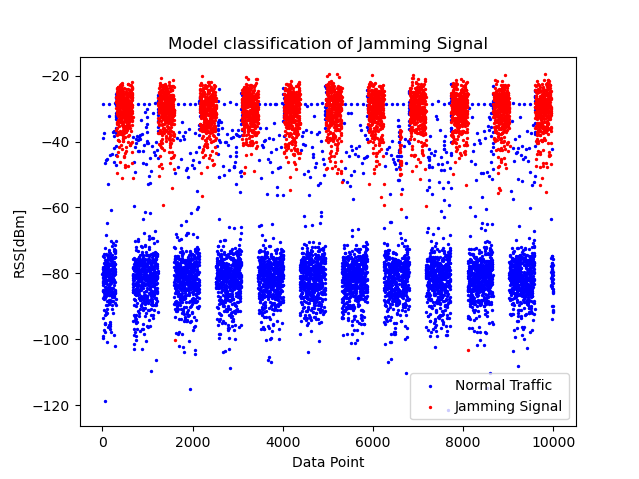
\includegraphics[width=\textwidth]{img/OnlyPeriodicJamming.png}
		\caption{Periodic Jamming classification.}
		\label{fig:periodicJammingClassification}
	\end{subfigure}
	\hfill
	\begin{subfigure}{0.49\textwidth}
		\centering
		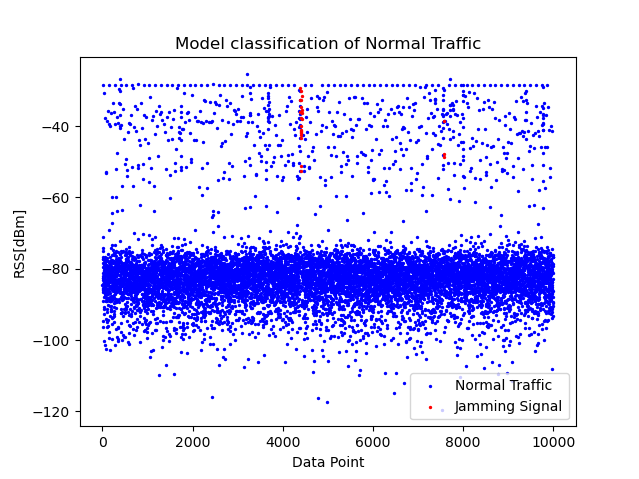
\includegraphics[width=\textwidth]{img/OnlyNormalTraffic.png}
		\caption{Normal Traffic classification.}
		\label{fig:normalTrafficClassification}
	\end{subfigure}
	\caption{Classification results of the proposed solution. The model is able to correctly classify periodic jamming and normal traffic with high accuracy.}
	\label{fig:proposedSolutionClassification}
\end{figure}

Our solution is able to achieve considerably better results in the classification of normal traffic and periodic jamming, while maintaining the same level of performance in the case of constant jamming.

%%%%%%%%%%%%%%%%%%%%%%%%%%%%%%%%%%%%%%%%%%
\section{Discussion}


In this article we analyzed whether it was possible to employ an Isolation Forest model to detect jamming attacks in a 6G drone scenario. We tuned the hyperparameters of the model and tested it against the default IF model. 
We achieved a considerable improvement in performance thanks to the tuning process (Section \ref{sec:standardModelTesting}), but despite the high recall and accuracy scores, the model experienced a high number of false positives, caused by the inherent noise of the dataset. 
To mitigate this issue, we proposed the integration of the IF model with a Majority Rule module (Section \ref{sec:majorityRuleModelTesting}). The \textit{window\_size} parameter of the MR module was tuned to provide the best performance.
The addition of the MR module proved extremely effective in reducing the number of false positives, greatly improving the model's precision. 

Integration of the MR module also impacted total classification time as shown in Figure \ref{fig:majority_rule_classification_time}, but the linear trend \cite{IsolationForestLiu} that we expected from the IF model was preserved, meaning that the classification time complexity was kept at $O(n)$. 
In our opinion, the trade-off between the increased classification time and the improved performance is justified, as the model is now much more reliable in a real-world scenario, where noise from the surrounding environment is almost always present.
The linear time complexity and low memory usage make the proposed solution suitable for a resource-constrained environment such as the analyzed 6G drone scenario.

As shown in Section \ref{sec:comparisonAgainstExistingSolution}, the proposed solution outperformed the solution proposed by \cite{JammingDetectionIoT-Hussain} in both the detection of periodic jamming and the classification of normal traffic, while achieving the same performance against constant jamming attacks. 
We believe that the importance of correct classification of normal traffic is often underestimated, as a high number of false positives can lead to the activation of resource-intensive countermeasures, even at times when they are not needed. 

\section{Conclusions}

In this article we analyzed the use of the Isolation Forest unsupervised machine learning algorithm for the detection of jamming attacks. We compared the performance of the base IF model against a version specifically tuned to detect jamming attacks. During the tuning phase, we paid particular attention to the computational impact of each parameter and tried to find the right balance between performance and efficiency. 
We then proposed the integration of a Majority Rule module to reduce the number of false positives caused by the inherent noise of the dataset. The MR module was tuned to provide the best performance and proved effective in mitigating the problem of false positives, while still maintaining a linear complexity in classification time.
We tested the model against a dataset that included normal traffic, constant jamming, and periodic jamming attacks, with an unbalanced number of normal traffic samples and jamming attack samples to better reflect a real-world scenario.
We compared the performance of the proposed solution against the solution proposed by \cite{JammingDetectionIoT-Hussain} and found that our solution outperformed the existing solution in both the detection of periodic jamming and the classification of normal traffic, while retaining the same performance against constant jamming attacks.


In a real world scenario, a 6G drone integrating the proposed solution would periodically run the tuning phase of the algorithm, selecting the best hyperparameters for the current environment. This could happen periodically or whenever there is a change in the environment caused by the drone moving to a different location. 
The dynamic tuning of the model would ensure that the parameters of the model are always optimized for the current environment, providing the best possible performance.
After the tuning phase, the drone would periodically sample incoming signals and classify them using the MR-integrated IF. If the model detects a jamming attack, the drone could activate built-in countermeasures like Frequency Hopping or Direct Sequence Spread Spectrum  to mitigate the effects of the attack. 

Future research could explore the model's performance against a broader range of jamming attacks types, including smart, reactive and random jamming, and evaluate the impact of real world noise on its accuracy.
Deploying the model on a drone would provide opportunity for real-world testing and valuable insights for further refinement.

As discussed in Section \ref{sec:DetectionMitigation}, devices integrated into 6G networks are expected to have a higher degree of sensing capabilities compared to current devices \cite{}. Thanks to the ability of the Isolation Forest to work on high dimensional data, the model could easily be expanded to include more classification features, which would improve its situational awareness and performance.
This could play a crucial role in addressing interference or signal shadowing patterns.

Furthermore, future work could include the investigation of the impact of adversarial settings, as this could offer insights into real-world performance as well as demonstrate adaptability to emerging 6G technologies.



%%%%%%%%%%%%%%%%%%%%%%%%%%%%%%%%%%%%%%%%%%
%\section{Patents}

%This Section is not mandatory, but may be added if there are patents resulting from the work reported in this manuscript.

%%%%%%%%%%%%%%%%%%%%%%%%%%%%%%%%%%%%%%%%%%
\vspace{6pt} 
%%%%%%%%%%%%%%%%%%%%%%%%%%%%%%%%%%%%%%%%%%
\authorcontributions{Conceptualization, Francesco Chiti and Sergio Cibecchini; methodology, Sergio Cibecchini; software, Sergio Cibecchini; validation, Francesco Chiti and Laura Pierucci; writing—original draft preparation, Sergio Cibecchini; writing—review and editing, Francesco Chiti and Laura Pierucci; visualization, Sergio Cibecchini; supervision, Francesco Chiti and Laura Pierucci. All authors have read and agreed to the published version of the manuscript.}

\funding{This research received no external funding.}

%\institutionalreview{In this section, you should add the Institutional Review Board Statement and approval number, if relevant to your study. You might choose to exclude this statement if the study did not require ethical approval. Please note that the Editorial Office might ask you for further information. Please add “The study was conducted in accordance with the Declaration of Helsinki, and approved by the Institutional Review Board (or Ethics Committee) of NAME OF INSTITUTE (protocol code XXX and date of approval).” for studies involving humans. OR “The animal study protocol was approved by the Institutional Review Board (or Ethics Committee) of NAME OF INSTITUTE (protocol code XXX and date of approval).” for studies involving animals. OR “Ethical review and approval were waived for this study due to REASON (please provide a detailed justification).” OR “Not applicable” for studies not involving humans or animals.}

%\informedconsent{Any research article describing a study involving humans should contain this statement. Please add ``Informed consent was obtained from all subjects involved in the study.'' OR ``Patient consent was waived due to REASON (please provide a detailed justification).'' OR ``Not applicable'' for studies not involving humans. You might also choose to exclude this statement if the study did not involve humans.

%Written informed consent for publication must be obtained from participating patients who can be identified (including by the patients themselves). Please state ``Written informed consent has been obtained from the patient(s) to publish this paper'' if applicable.}

\dataavailability{The dataset used in this study is openly available and provided by the authors of \cite{JammingDetectionIoT-Hussain} at the following URL: \url{https://github.com/AMHD/Jamming-Detection-in-IoT-Wireless-Networks-An-Edge-AI-Based-Approach}. The code for the tests and the jamming detection model developed in this study is available in the following repository: \url{https://github.com/cibecs/JammingAttacksAnomalyDetection.git}.}

\acknowledgments{This work was partially supported by the European Union under the Italian National Recovery and Resilience Plan (NRRP) of NextGenerationEU, in partnership with the project “Telecommunications of the Future” (PE00000001—program “RESTART”). Additionally, this article publication is based upon work from COST Action CA22168 for "Physical Layer Security for Trustworthy and Resilient 6G Systems (6G-PHYSEC)," supported by COST (European Cooperation in Science and Technology).}

\conflictsofinterest{The authors declare no conflicts of interest.} 

\abbreviations{Abbreviations}{
The following abbreviations are used in this manuscript:\\

\noindent 
\begin{tabular}{@{}ll}
SDN & Software Defined Networks\\
UAVs & Unmanned Aerial Vehicles \\
3GPP & 3rd Generation Partnership Project \\
ML & Machine Learning \\
V2X & Vehicle to Everything \\
FPV & First Person View \\
BS & Base Station \\
MR & Majority Rule \\
DOS & Denial Of Service \\
SNR & Signal to Noise Ratio \\
RSSI & Received Signal Strength Indicator \\
PDR & Packet Delivery Ratio \\
CIA & Confidentiality, Integrity, Availability \\
IoT & Internet of Things \\
AI & Artificial Intelligence \\
DSSS & Direct Sequence Spread Spectrum \\
FHSS & Frequency Hopping Spread Spectrum \\
OSI & Open Systems Interconnection \\
dBm & Decibel-milliwatts \\
IF & Isolation Forest \\
CNN & Convolutional Neural Network \\
RSV & Relative Speed Variation \\


\end{tabular}
}


\begin{adjustwidth}{-\extralength}{0cm}
%\printendnotes[custom] % Un-comment to print a list of endnotes

\reftitle{References}

%=====================================
% References, variant B: internal bibliography
%=====================================
\begin{thebibliography}{999}

\bibitem[Taylor(2024)]{5GStatisticsTaylor}
5G - statistics \& facts. Available online: \url{https://www.statista.com/topics/3447/5g/topicOverview} (accessed on 13 September 2024).

\bibitem[Chiti et al.(2021)]{ChFaPi21}
Chiti, F. and Fantacci, R. and Pierucci, L. A Green Routing Protocol with Wireless Power Transfer for Internet of Things. {\em Journal of Sensor and Actuator Networks} {\bf 2021}, {\em 10}, {\em 1}. \url{https://doi.org/10.3390/jsan10010006}.

\bibitem[Letaief et al.(2019)]{6GRoadmapLetaief}
Letaief, K.B.; Chen, W.; Shi, Y.; Zhang, J.; AI, B. The Roadmap to 6G: AI Empowered Wireless Networks. {\em IEEE Communications Magazine} {\bf 2019}, {\em 57}, 84--90. \url{https://doi.org/10.1109/MCOM.2019.1900271}.

\bibitem[Chiti et al.(2016)]{LoPu16}
Chiti, F. and Fantacci, R. and Loreti, M. and Pugliese, R. Context-aware wireless mobile autonomic computing and communications: research trends and emerging applications. {\em IEEE Wireless Communications} {\bf 2016}, {\em 23}, {\em 2}, 86--92. \url{https://10.1109/MWC.2016.7462489}.

\bibitem[Lyamin et al.(2018)]{VANETsAI-Lyamin}
Lyamin, N.; Samuylov, A.; Gaidamaka, Y.; Vinel, A.; Koucheryavy, Y. AI-Based Malicious Network Traffic Detection in VANETs. {\em IEEE Network} {\bf 2018}, {\em 32}, 15--21. \url{https://doi.org/10.1109/MNET.2018.1800074}.

\bibitem[Arjoune et al.(2020)]{JammingDetectionML-Arjoune}
Arjoune, Y.; Salahdine, F.; Islam, M.S.; Ghribi, E.; Kaabouch, N. A Novel Jamming Attacks Detection Approach Based on Machine Learning for Wireless Communication. In Proceedings of the 2020 International Conference on Information Networking (ICOIN), Barcelona, Spain, 2020; pp. 459--464. https://doi.org/10.1109/ICOIN48656.2020.9016462.

\bibitem[Karagiannis and Argyriou(2018)]{JammingDetectionRF-Karagiannis}
Karagiannis, D.; Argyriou, A. Jamming attack detection in a pair of RF communicating vehicles using unsupervised machine learning. {\em Vehicular Communications} {\bf 2018}, {\em 13}, 56--63. https://doi.org/10.1016/j.vehcom.2018.05.001. Available online: \url{https://www.sciencedirect.com/science/article/pii/S221420961730222X}.

\bibitem[Greco et al.(2021)]{JammingDetectionDrones-Greco}
Greco, C.; Pace, P.; Basagni, S.; Fortino, G. Jamming detection at the edge of drone networks using Multi-layer Perceptrons and Decision Trees. {\em Applied Soft Computing} {\bf 2021}, {\em 111}, 107806. https://doi.org/10.1016/j.asoc.2021.107806. Available online: \url{https://www.sciencedirect.com/science/article/pii/S1568494621007274}.

\bibitem[Hussain et al.(2023)]{JammingDetectionIoT-Hussain}
Hussain, A.; Zhang, M.; Bhatia, S.; Cheng, L. Jamming Detection in IoT Wireless Networks: An Edge-AI Based Approach. In Proceedings of the 12th International Conference on the Internet of Things, IoT ’22; Association for Computing Machinery: Delft, Netherlands, 2023; pp. 57--64. ISBN: 9781450396653. \url{https://doi.org/10.1145/3567445.3567456}.

\bibitem[Zuo et al.(2021)]{GPSSpoofingDetection-Zuo}
Zuo, S.; Liu, Y.; Zhang, D.; Xin, P.; Liu, T. Detection of GPS Spoofing Attacks Based on Isolation Forest. In Proceedings of the 2021 IEEE 9th International Conference on Information, Communication and Networks (ICICN), Xi'an, China, 2021; pp. 357--361. \url{https://doi.org/10.1109/ICICN52636.2021.9673863}.

\bibitem[Hong et al.(2023)]{HybridJammingDetection-Hong}
Hong, S.; Kim, K.; Lee, S.-H. A Hybrid Jamming Detection Algorithm for Wireless Communications: Simultaneous Classification of Known Attacks and Detection of Unknown Attacks. {\em IEEE Communications Letters} {\bf 2023}, {\em 27}, 1769--1773. \url{https://doi.org/10.1109/LCOMM.2023.3275694}.

\bibitem[EuropeanCommission(2024)]{DronesEC}
Unmanned aircraft (drones). Available online: \url{https://transport.ec.europa.eu/transport-modes/air/aviation-safety/unmanned-aircraft-drones_en} (accessed on 13 September 2024).

\bibitem[Laricchia(2024)]{DronesStatisticsLaricchia}
Laricchia, F. Consumer and commercial drones - statistics and facts. Available online: \url{https://www.statista.com/topics/7939/drones/\#topicOverview} (accessed on 13 September 2024).

\bibitem[Sultan(2018)]{5GV2XSultan}
Sultan, A. Study on enhancement of 3GPP support for 5G V2X services. Tech. Rep. {\em 3GPP}, 2018.

\bibitem[Hassija et al.(2021)]{DroneCommHassija}
Hassija, V.; Kumar, R.; Gupta, H.; Singh, S.; Sharma, P. Fast, Reliable, and Secure Drone Communication: A Comprehensive Survey. {\em IEEE Communications Surveys and Tutorials} {\bf 2021}, {\em 23}, 2802--2832. \url{https://doi.org/10.1109/COMST.2021.3097916}.

\bibitem[Cawthra(2020)]{DataIntegrityCawthra}
Cawthra, J. Data Integrity: Detecting and Responding to Ransomware and Other Destructive Events. {\em NIST Special Publication} {\bf 2020}, {\em 1800-26A}.

\bibitem[Boualouache and Engel(2023)]{MLMisbehavior5GBoualouache}
Boualouache, A.; Engel, T. A Survey on Machine Learning-Based Misbehavior Detection Systems for 5G and Beyond Vehicular Networks. {\em IEEE Communications Surveys and Tutorials} {\bf 2023}, {\em 25}, 1128--1172. \url{https://doi.org/10.1109/COMST.2023.3236448}.

\bibitem[Feng and Haykin(2019)]{AntiJammingV2V-Feng}
Feng, S.; Haykin, S. Cognitive Risk Control for Anti-Jamming V2V Communications in Autonomous Vehicle Networks. {\em IEEE Transactions on Vehicular Technology} {\bf 2019}, {\em 68}, 9920--9934. \url{https://doi.org/10.1109/TVT.2019.2935999}.

\bibitem[Owano(2024)]{RQ170DroneOwano}
Owano, N. RQ-170 drone's ambush facts spilled by Iranian engineer. Available online: \url{https://phys.org/news/2011-12-rq-drone-ambush-facts-iranian.html} (accessed on 14 September 2024).

\bibitem[Chorti et al.(2022)]{6GSecurity-Chorti}
Chorti, A.; Hollanti, C.; Koorapaty, H.; Poor, H.V. Context-Aware Security for 6G Wireless: The Role of Physical Layer Security. {\em IEEE Communications Standards Magazine} {\bf 2022}, {\em 6}, 102--108. https://doi.org/10.1109/MCOMSTD.0001.2000082.

\bibitem[Sciancalepore et al.(2023)]{JammingDetection-Sciancalepore}
Sciancalepore, S.; Kusters, F.; Abdelhadi, N.K.; Oligeri, G. Jamming Detection in Low-BER Mobile Indoor Scenarios via Deep Learning. {\em arXiv} {\bf 2023}, eprint: 2306.10912. Available online: \url{https://arxiv.org/abs/2306.10912}.

\bibitem[Liu et al.(2008)]{IsolationForestLiu}
Liu, F.T.; Ting, K.M.; Zhou, Z.-H. Isolation Forest. In Proceedings of the 2008 Eighth IEEE International Conference on Data Mining, Pisa, Italy, 2008; pp. 413--422. \url{https://doi.org/10.1109/ICDM.2008.17}.

\bibitem[Scikit-learn(2024)]{IsolationForestScikitLearn}
Scikit-learn: Isolation Forest. Available online: \url{https://scikit-learn.org/stable/modules/generated/sklearn.ensemble.IsolationForest.html} (accessed on 14 September 2024).

\end{thebibliography}

% If authors have biography, please use the format below
%\section*{Short Biography of Authors}
%\bio
%{\raisebox{-0.35cm}{\includegraphics[width=3.5cm,height=5.3cm,clip,keepaspectratio]{Definitions/author1.pdf}}}
%{\textbf{Firstname Lastname} Biography of first author}
%
%\bio
%{\raisebox{-0.35cm}{\includegraphics[width=3.5cm,height=5.3cm,clip,keepaspectratio]{Definitions/author2.jpg}}}
%{\textbf{Firstname Lastname} Biography of second author}

% For the MDPI journals use author-date citation, please follow the formatting guidelines on http://www.mdpi.com/authors/references
% To cite two works by the same author: \citeauthor{ref-journal-1a} (\citeyear{ref-journal-1a}, \citeyear{ref-journal-1b}). This produces: Whittaker (1967, 1975)
% To cite two works by the same author with specific pages: \citeauthor{ref-journal-3a} (\citeyear{ref-journal-3a}, p. 328; \citeyear{ref-journal-3b}, p.475). This produces: Wong (1999, p. 328; 2000, p. 475)


\PublishersNote{}
\end{adjustwidth}
\end{document}

